\documentclass[]{article}
\usepackage{lmodern}
\usepackage{amssymb,amsmath}
\usepackage{ifxetex,ifluatex}
\usepackage{fixltx2e} % provides \textsubscript
\ifnum 0\ifxetex 1\fi\ifluatex 1\fi=0 % if pdftex
  \usepackage[T1]{fontenc}
  \usepackage[utf8]{inputenc}
\else % if luatex or xelatex
  \ifxetex
    \usepackage{mathspec}
  \else
    \usepackage{fontspec}
  \fi
  \defaultfontfeatures{Ligatures=TeX,Scale=MatchLowercase}
\fi
% use upquote if available, for straight quotes in verbatim environments
\IfFileExists{upquote.sty}{\usepackage{upquote}}{}
% use microtype if available
\IfFileExists{microtype.sty}{%
\usepackage{microtype}
\UseMicrotypeSet[protrusion]{basicmath} % disable protrusion for tt fonts
}{}
\usepackage[margin=1in]{geometry}
\usepackage{hyperref}
\hypersetup{unicode=true,
            pdftitle={R Homework Assignment},
            pdfauthor={Jeeban Panthi, Mamoon Y. Ismail, Tiare Fridrich},
            pdfborder={0 0 0},
            breaklinks=true}
\urlstyle{same}  % don't use monospace font for urls
\usepackage{color}
\usepackage{fancyvrb}
\newcommand{\VerbBar}{|}
\newcommand{\VERB}{\Verb[commandchars=\\\{\}]}
\DefineVerbatimEnvironment{Highlighting}{Verbatim}{commandchars=\\\{\}}
% Add ',fontsize=\small' for more characters per line
\usepackage{framed}
\definecolor{shadecolor}{RGB}{248,248,248}
\newenvironment{Shaded}{\begin{snugshade}}{\end{snugshade}}
\newcommand{\KeywordTok}[1]{\textcolor[rgb]{0.13,0.29,0.53}{\textbf{#1}}}
\newcommand{\DataTypeTok}[1]{\textcolor[rgb]{0.13,0.29,0.53}{#1}}
\newcommand{\DecValTok}[1]{\textcolor[rgb]{0.00,0.00,0.81}{#1}}
\newcommand{\BaseNTok}[1]{\textcolor[rgb]{0.00,0.00,0.81}{#1}}
\newcommand{\FloatTok}[1]{\textcolor[rgb]{0.00,0.00,0.81}{#1}}
\newcommand{\ConstantTok}[1]{\textcolor[rgb]{0.00,0.00,0.00}{#1}}
\newcommand{\CharTok}[1]{\textcolor[rgb]{0.31,0.60,0.02}{#1}}
\newcommand{\SpecialCharTok}[1]{\textcolor[rgb]{0.00,0.00,0.00}{#1}}
\newcommand{\StringTok}[1]{\textcolor[rgb]{0.31,0.60,0.02}{#1}}
\newcommand{\VerbatimStringTok}[1]{\textcolor[rgb]{0.31,0.60,0.02}{#1}}
\newcommand{\SpecialStringTok}[1]{\textcolor[rgb]{0.31,0.60,0.02}{#1}}
\newcommand{\ImportTok}[1]{#1}
\newcommand{\CommentTok}[1]{\textcolor[rgb]{0.56,0.35,0.01}{\textit{#1}}}
\newcommand{\DocumentationTok}[1]{\textcolor[rgb]{0.56,0.35,0.01}{\textbf{\textit{#1}}}}
\newcommand{\AnnotationTok}[1]{\textcolor[rgb]{0.56,0.35,0.01}{\textbf{\textit{#1}}}}
\newcommand{\CommentVarTok}[1]{\textcolor[rgb]{0.56,0.35,0.01}{\textbf{\textit{#1}}}}
\newcommand{\OtherTok}[1]{\textcolor[rgb]{0.56,0.35,0.01}{#1}}
\newcommand{\FunctionTok}[1]{\textcolor[rgb]{0.00,0.00,0.00}{#1}}
\newcommand{\VariableTok}[1]{\textcolor[rgb]{0.00,0.00,0.00}{#1}}
\newcommand{\ControlFlowTok}[1]{\textcolor[rgb]{0.13,0.29,0.53}{\textbf{#1}}}
\newcommand{\OperatorTok}[1]{\textcolor[rgb]{0.81,0.36,0.00}{\textbf{#1}}}
\newcommand{\BuiltInTok}[1]{#1}
\newcommand{\ExtensionTok}[1]{#1}
\newcommand{\PreprocessorTok}[1]{\textcolor[rgb]{0.56,0.35,0.01}{\textit{#1}}}
\newcommand{\AttributeTok}[1]{\textcolor[rgb]{0.77,0.63,0.00}{#1}}
\newcommand{\RegionMarkerTok}[1]{#1}
\newcommand{\InformationTok}[1]{\textcolor[rgb]{0.56,0.35,0.01}{\textbf{\textit{#1}}}}
\newcommand{\WarningTok}[1]{\textcolor[rgb]{0.56,0.35,0.01}{\textbf{\textit{#1}}}}
\newcommand{\AlertTok}[1]{\textcolor[rgb]{0.94,0.16,0.16}{#1}}
\newcommand{\ErrorTok}[1]{\textcolor[rgb]{0.64,0.00,0.00}{\textbf{#1}}}
\newcommand{\NormalTok}[1]{#1}
\usepackage{graphicx,grffile}
\makeatletter
\def\maxwidth{\ifdim\Gin@nat@width>\linewidth\linewidth\else\Gin@nat@width\fi}
\def\maxheight{\ifdim\Gin@nat@height>\textheight\textheight\else\Gin@nat@height\fi}
\makeatother
% Scale images if necessary, so that they will not overflow the page
% margins by default, and it is still possible to overwrite the defaults
% using explicit options in \includegraphics[width, height, ...]{}
\setkeys{Gin}{width=\maxwidth,height=\maxheight,keepaspectratio}
\IfFileExists{parskip.sty}{%
\usepackage{parskip}
}{% else
\setlength{\parindent}{0pt}
\setlength{\parskip}{6pt plus 2pt minus 1pt}
}
\setlength{\emergencystretch}{3em}  % prevent overfull lines
\providecommand{\tightlist}{%
  \setlength{\itemsep}{0pt}\setlength{\parskip}{0pt}}
\setcounter{secnumdepth}{0}
% Redefines (sub)paragraphs to behave more like sections
\ifx\paragraph\undefined\else
\let\oldparagraph\paragraph
\renewcommand{\paragraph}[1]{\oldparagraph{#1}\mbox{}}
\fi
\ifx\subparagraph\undefined\else
\let\oldsubparagraph\subparagraph
\renewcommand{\subparagraph}[1]{\oldsubparagraph{#1}\mbox{}}
\fi

%%% Use protect on footnotes to avoid problems with footnotes in titles
\let\rmarkdownfootnote\footnote%
\def\footnote{\protect\rmarkdownfootnote}

%%% Change title format to be more compact
\usepackage{titling}

% Create subtitle command for use in maketitle
\newcommand{\subtitle}[1]{
  \posttitle{
    \begin{center}\large#1\end{center}
    }
}

\setlength{\droptitle}{-2em}
  \title{R Homework Assignment}
  \pretitle{\vspace{\droptitle}\centering\huge}
  \posttitle{\par}
  \author{Jeeban Panthi, Mamoon Y. Ismail, Tiare Fridrich}
  \preauthor{\centering\large\emph}
  \postauthor{\par}
  \predate{\centering\large\emph}
  \postdate{\par}
  \date{2018-04-01}


\begin{document}
\maketitle

\textbf{BOLD}

\emph{ITALICS}

1- The backticks (`) indicate code

2- r indicates R code

3- In-line code: is how to include r code results into text

The version of R is 3.4.3

4- It’s usually best to give each code chunk a name, like chunk\_name
```\{r chunk\_name\}

5- echo=FALSE indicates that the code will not be shown in the final
document like this ```\{r chunk\_name, echo=FALSE\}

6- Use results=``hide'' to hide the results/output (but here the code
would still be displayed), ```\{r chunk\_name, results=``hide''\}

7- Use include=FALSE to have the chunk evaluated, but neither the code
nor its output displayed, ```\{r chunk\_name, include=FALSE\}

8- For figures, you’ll want to use options like fig.width and
fig.height. For example: \{r scatterplot, fig.width=8, fig.height=6\}.
Note that if include=FALSE, all of the code, results, and figures will
be suppressed. If include=TRUE and results=``hide'', the results will be
hidden but figures will still be shown. To hide the figures, use
fig.show=``hide''. NOTE: results=hide is wrong; you need
results=``hide''.

9- Global chunk options: use the same set of chunk options throughout a
document to avoid retype it in every chunk, so you want to set some
global chunk options at the top of your document. For example, I might
use include=FALSE or at least echo=FALSE globally for a report to a
scientific collaborator who wouldn’t want to see all of the code. And
I might want something like fig.width=12 and fig.height=6 if I generally
want those sizes for my figures.

10- If you want a particular chunk to have a different behavior, for
example, to have a different figure height, you’d specify a different
option within that chunk. For example: \{r a\_taller\_figure,
fig.height=32\}.

\subsubsection{Loading librarry}\label{loading-librarry}

A chunk needed to load the library

\begin{Shaded}
\begin{Highlighting}[]
\KeywordTok{library}\NormalTok{(tidyverse)}
\end{Highlighting}
\end{Shaded}

\begin{verbatim}
## -- Attaching packages -------------------------------------------- tidyverse 1.2.1 --
\end{verbatim}

\begin{verbatim}
## v ggplot2 2.2.1     v purrr   0.2.4
## v tibble  1.4.2     v dplyr   0.7.4
## v tidyr   0.8.0     v stringr 1.3.0
## v readr   1.1.1     v forcats 0.3.0
\end{verbatim}

\begin{verbatim}
## -- Conflicts ----------------------------------------------- tidyverse_conflicts() --
## x dplyr::filter() masks stats::filter()
## x dplyr::lag()    masks stats::lag()
\end{verbatim}

\begin{Shaded}
\begin{Highlighting}[]
\KeywordTok{library}\NormalTok{(ggplot2)}
\KeywordTok{library}\NormalTok{(lubridate)}
\end{Highlighting}
\end{Shaded}

\begin{verbatim}
## 
## Attaching package: 'lubridate'
\end{verbatim}

\begin{verbatim}
## The following object is masked from 'package:base':
## 
##     date
\end{verbatim}

\begin{Shaded}
\begin{Highlighting}[]
\KeywordTok{library}\NormalTok{(gridExtra)}
\end{Highlighting}
\end{Shaded}

\begin{verbatim}
## Warning: package 'gridExtra' was built under R version 3.4.4
\end{verbatim}

\begin{verbatim}
## 
## Attaching package: 'gridExtra'
\end{verbatim}

\begin{verbatim}
## The following object is masked from 'package:dplyr':
## 
##     combine
\end{verbatim}

\begin{Shaded}
\begin{Highlighting}[]
\KeywordTok{library}\NormalTok{(dplyr)}
\KeywordTok{library}\NormalTok{(ggpubr)}
\end{Highlighting}
\end{Shaded}

\begin{verbatim}
## Warning: package 'ggpubr' was built under R version 3.4.4
\end{verbatim}

\begin{verbatim}
## Loading required package: magrittr
\end{verbatim}

\begin{verbatim}
## 
## Attaching package: 'magrittr'
\end{verbatim}

\begin{verbatim}
## The following object is masked from 'package:purrr':
## 
##     set_names
\end{verbatim}

\begin{verbatim}
## The following object is masked from 'package:tidyr':
## 
##     extract
\end{verbatim}

\begin{Shaded}
\begin{Highlighting}[]
\KeywordTok{library}\NormalTok{(Hmisc)}
\end{Highlighting}
\end{Shaded}

\begin{verbatim}
## Warning: package 'Hmisc' was built under R version 3.4.4
\end{verbatim}

\begin{verbatim}
## Loading required package: lattice
\end{verbatim}

\begin{verbatim}
## Loading required package: survival
\end{verbatim}

\begin{verbatim}
## Loading required package: Formula
\end{verbatim}

\begin{verbatim}
## 
## Attaching package: 'Hmisc'
\end{verbatim}

\begin{verbatim}
## The following objects are masked from 'package:dplyr':
## 
##     src, summarize
\end{verbatim}

\begin{verbatim}
## The following objects are masked from 'package:base':
## 
##     format.pval, units
\end{verbatim}

\subsection{Global Options}\label{global-options}

\begin{Shaded}
\begin{Highlighting}[]
\CommentTok{#These are default settings eg fig size or whether you print code}
\NormalTok{knitr}\OperatorTok{::}\NormalTok{opts_chunk}\OperatorTok{$}\KeywordTok{set}\NormalTok{(}\DataTypeTok{echo =} \OtherTok{TRUE}\NormalTok{, }\DataTypeTok{warning=}\OtherTok{FALSE}\NormalTok{, }\DataTypeTok{message=}\OtherTok{FALSE}\NormalTok{,}
                      \DataTypeTok{fig.width=}\DecValTok{12}\NormalTok{, }\DataTypeTok{fig.height=}\DecValTok{8}\NormalTok{, }\DataTypeTok{fig.path=}\StringTok{'figs/'}\NormalTok{)}
\end{Highlighting}
\end{Shaded}

\subsection{SURVEYS}\label{surveys}

This is a survey data that has been collected about animal species.

\subsubsection{Reading Data}\label{reading-data}

Reading Colected data into a file called survey

\begin{Shaded}
\begin{Highlighting}[]
\NormalTok{surveys <-}\StringTok{ }\KeywordTok{read_csv}\NormalTok{(}\StringTok{"https://ndownloader.figshare.com/files/2292169"}\NormalTok{)}
\NormalTok{surveys_NAsrem <-}\StringTok{ }\NormalTok{surveys }\OperatorTok\StringTok{ }\KeywordTok{filter}\NormalTok{(}\OperatorTok{!}\KeywordTok{is.na}\NormalTok{(weight), }\OperatorTok{!}\KeywordTok{is.na}\NormalTok{(hindfoot_length), }\OperatorTok{!}\KeywordTok{is.na}\NormalTok{(sex), species_id }\OperatorTok{!=}\StringTok{ ""}\NormalTok{)}
\end{Highlighting}
\end{Shaded}

\subsection{Plotting}\label{plotting}

Add plots of different relations

\subsection{Session Info:}\label{session-info}

Include “session info” in your document, preferably at the bottom:
that lists the version of R that you’re using plus all of the packages
you’ve loaded

These are the packages we need to deal with

\section{1. Relationship between sex and hindfoot
length}\label{relationship-between-sex-and-hindfoot-length}

\begin{Shaded}
\begin{Highlighting}[]
\KeywordTok{ggplot}\NormalTok{(surveys_NAsrem, }\KeywordTok{aes}\NormalTok{(}\DataTypeTok{x=}\NormalTok{sex, }\DataTypeTok{y=}\NormalTok{hindfoot_length))}\OperatorTok{+}
\StringTok{  }\KeywordTok{geom_boxplot}\NormalTok{(}\DataTypeTok{alpha =} \DecValTok{1}\NormalTok{,}\DataTypeTok{color=}\StringTok{'blue'}\NormalTok{)}\OperatorTok{+}\KeywordTok{xlab}\NormalTok{(}\StringTok{'Sex'}\NormalTok{)}\OperatorTok{+}\KeywordTok{ylab}\NormalTok{(}\StringTok{'Length of hindfoot (inch)'}\NormalTok{)}\OperatorTok{+}
\StringTok{  }\KeywordTok{stat_summary}\NormalTok{(}\DataTypeTok{fun.y=}\NormalTok{mean, }\DataTypeTok{color=}\StringTok{"red"}\NormalTok{, }\DataTypeTok{geom=}\StringTok{"point"}\NormalTok{, }\DataTypeTok{shape=}\DecValTok{15}\NormalTok{, }\DataTypeTok{size=}\DecValTok{1}\NormalTok{,}\DataTypeTok{show_guide =}\NormalTok{ T, }\DataTypeTok{show.legend =}\NormalTok{ T) }\OperatorTok{+}\StringTok{ }\KeywordTok{theme_bw}\NormalTok{()}
\end{Highlighting}
\end{Shaded}

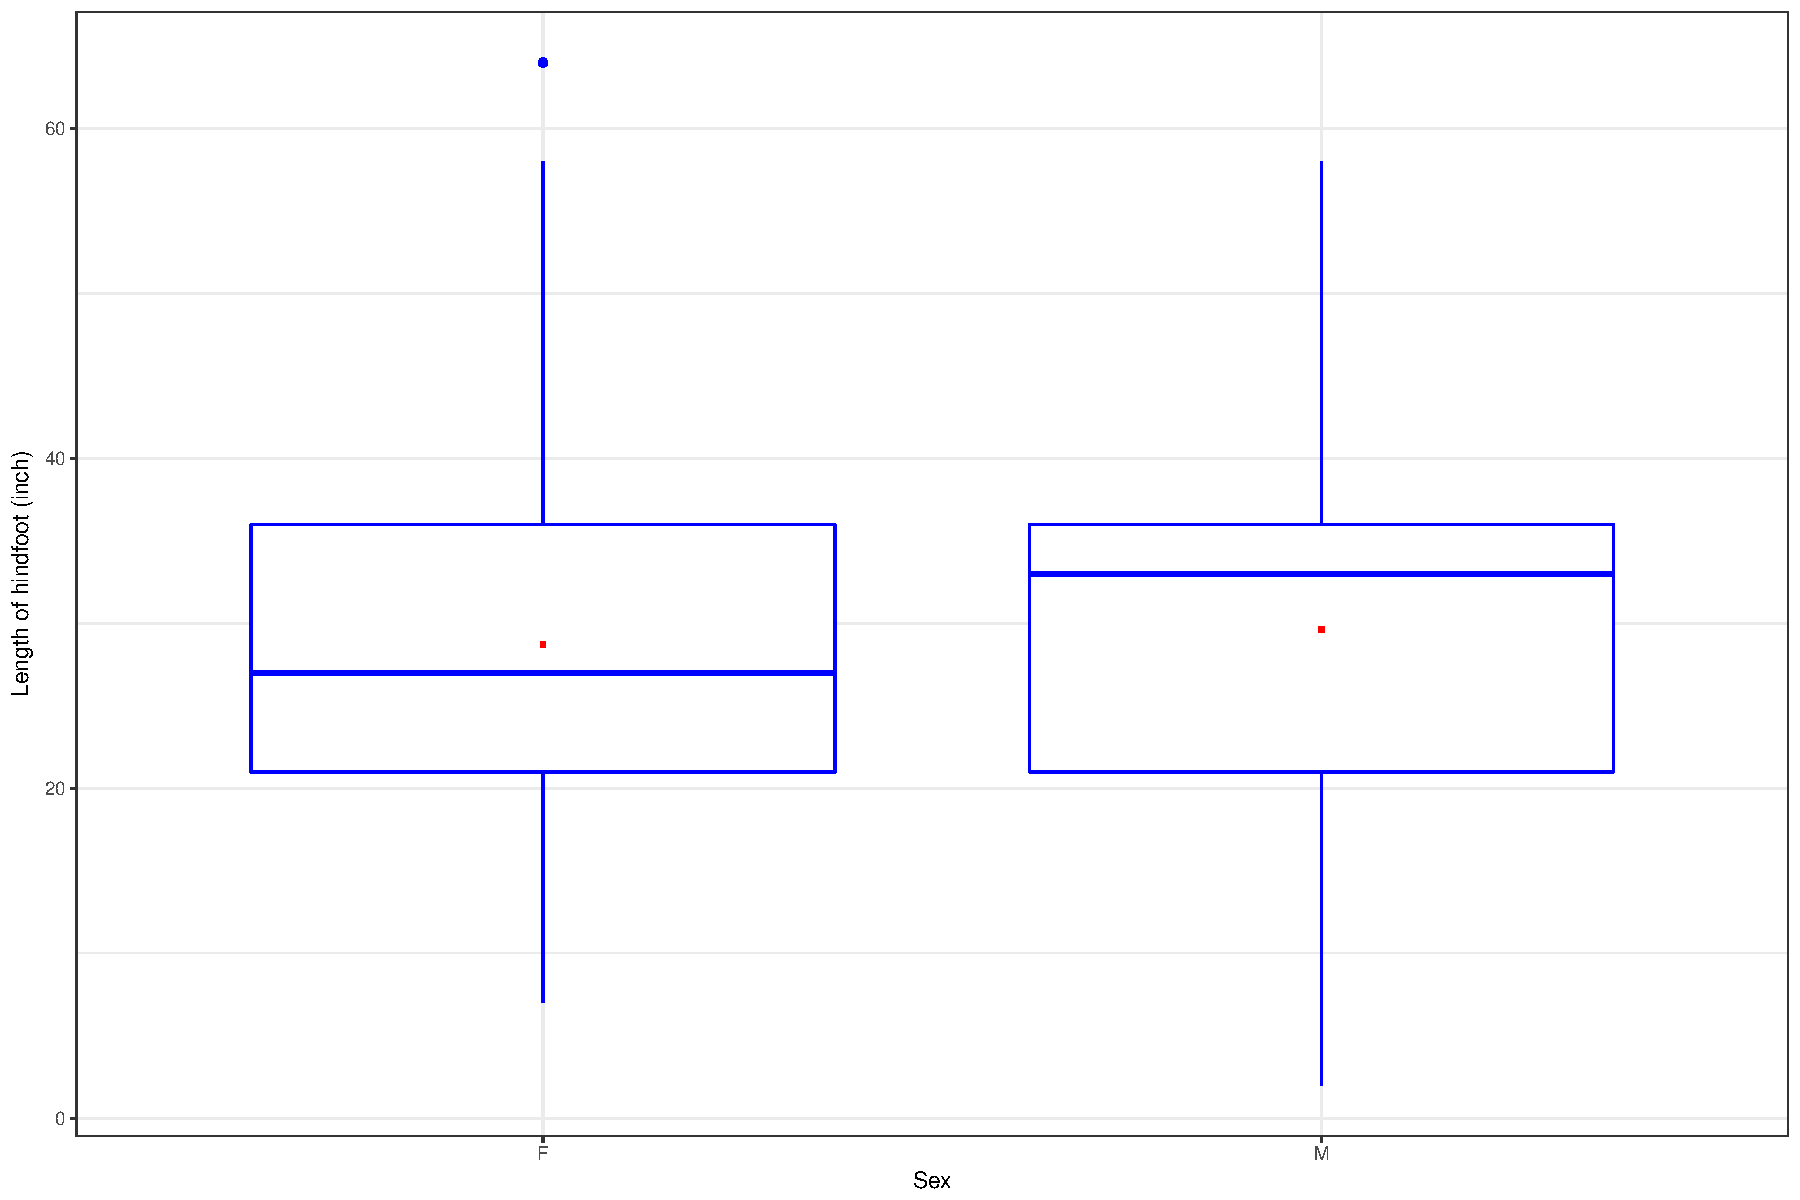
\includegraphics{figs/relationship between sex and hindfoot length boxplot-1.pdf}
Figure 1: Hindfoot length for male and female. The red dot indicates the
mean (average) hindfoot length.

\section{2. Number of individuals of each of the species classfied by
sex}\label{number-of-individuals-of-each-of-the-species-classfied-by-sex}

\begin{Shaded}
\begin{Highlighting}[]
\KeywordTok{ggplot}\NormalTok{(surveys_NAsrem, }\KeywordTok{aes}\NormalTok{(species_id))}\OperatorTok{+}\KeywordTok{geom_bar}\NormalTok{(}\KeywordTok{aes}\NormalTok{(}\DataTypeTok{fill=}\NormalTok{sex))}\OperatorTok{+}
\StringTok{  }\KeywordTok{ylab}\NormalTok{(}\StringTok{'Number of individuals recorded'}\NormalTok{)}\OperatorTok{+}\KeywordTok{xlab}\NormalTok{(}\StringTok{'Species ID'}\NormalTok{)}\OperatorTok{+}\KeywordTok{theme}\NormalTok{(}\DataTypeTok{axis.text.x =} \KeywordTok{element_text}\NormalTok{(}\DataTypeTok{angle =} \DecValTok{90}\NormalTok{)) }
\end{Highlighting}
\end{Shaded}

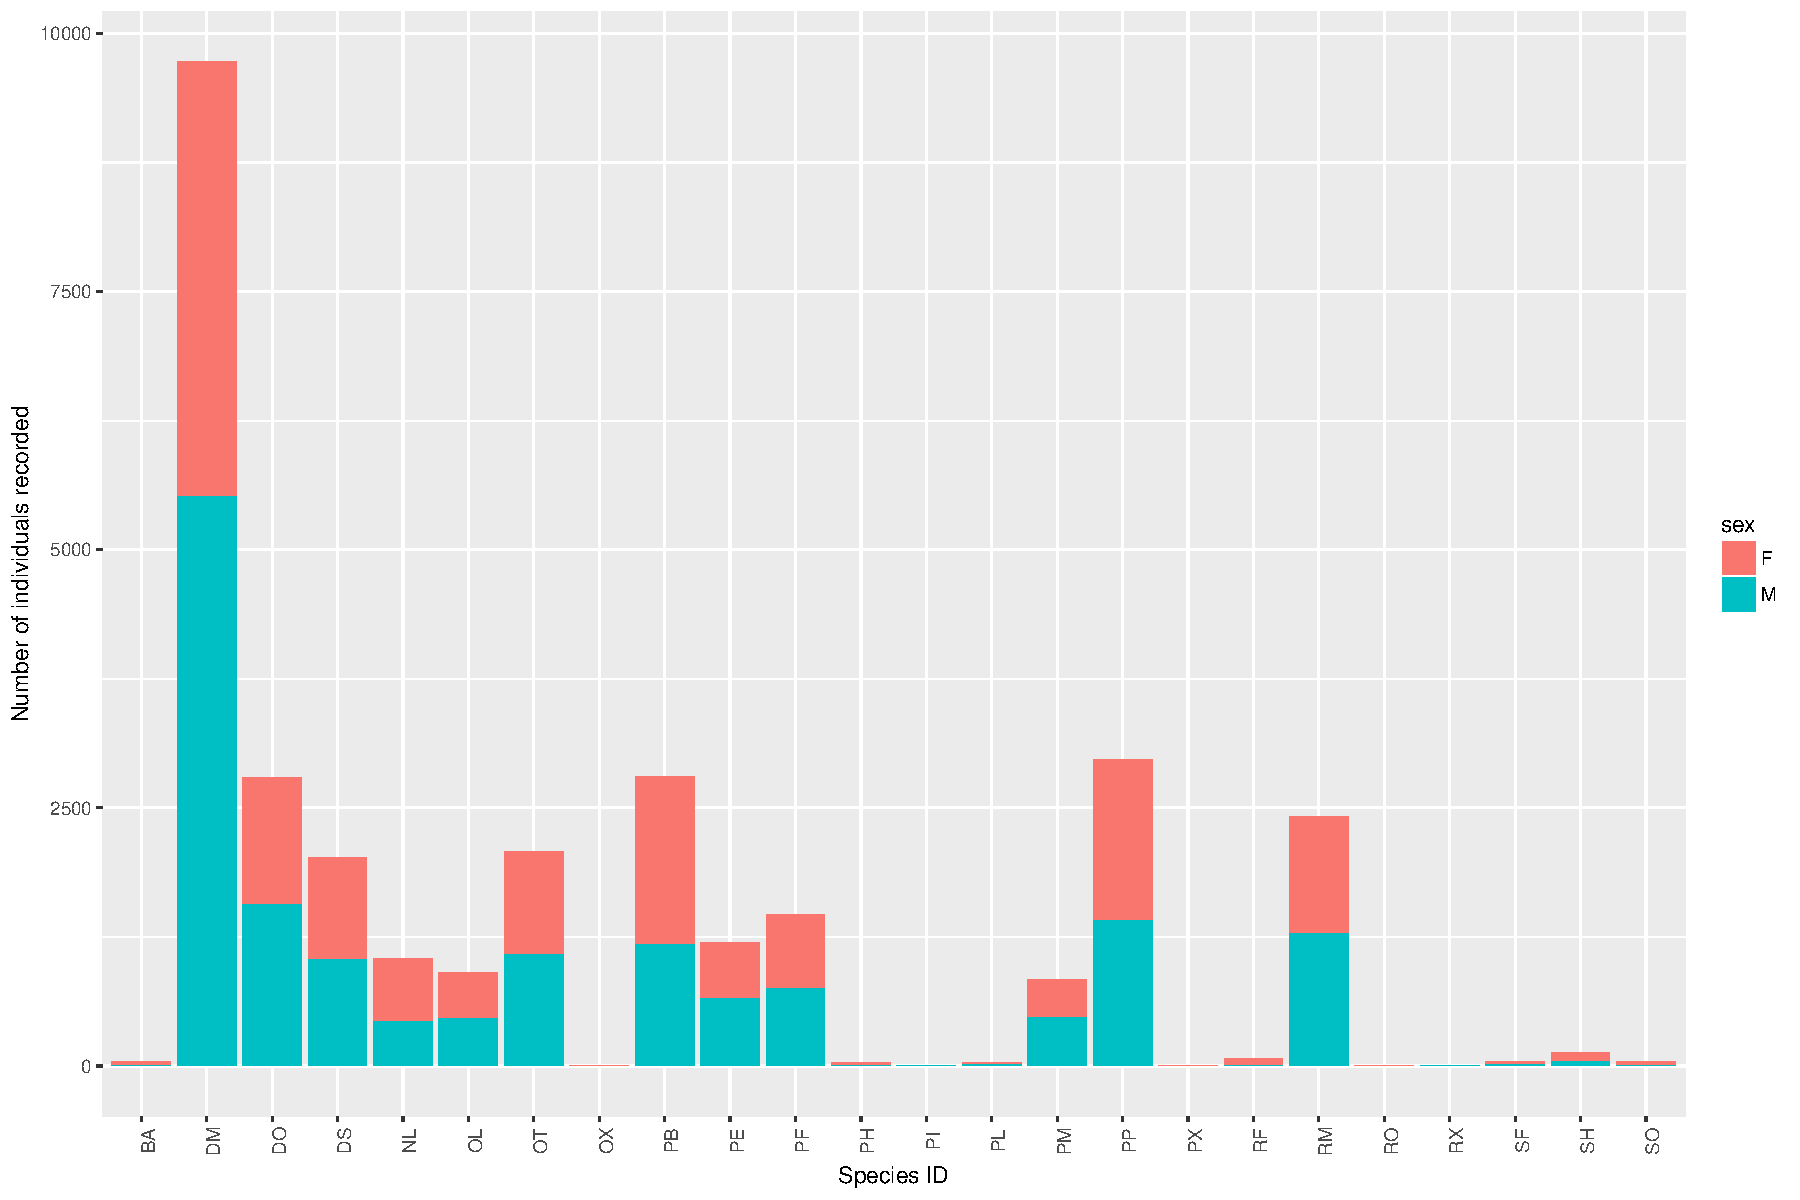
\includegraphics{figs/Individuals_per_species_sex-1.pdf} Figure 2:
Number of individuals of each of the species classfied by sex

\section{3. Correlationship between weight and hindfoot
length}\label{correlationship-between-weight-and-hindfoot-length}

\begin{Shaded}
\begin{Highlighting}[]
\KeywordTok{ggscatter}\NormalTok{(surveys_NAsrem, }\DataTypeTok{x =} \StringTok{"weight"}\NormalTok{, }\DataTypeTok{y =} \StringTok{"hindfoot_length"}\NormalTok{, }\DataTypeTok{color =} \StringTok{"black"}\NormalTok{, }\DataTypeTok{shape =} \DecValTok{21}\NormalTok{, }\DataTypeTok{size =} \DecValTok{2}\NormalTok{, }\DataTypeTok{add =} \StringTok{"reg.line"}\NormalTok{, }\DataTypeTok{conf.int =} \OtherTok{TRUE}\NormalTok{, }\DataTypeTok{cor.coef =} \OtherTok{TRUE}\NormalTok{, }\DataTypeTok{cor.method =} \StringTok{"pearson"}\NormalTok{,  }\DataTypeTok{xlab =} \StringTok{"Hindfoot Length (inch)"}\NormalTok{, }\DataTypeTok{ylab =} \StringTok{"Weight (gram)"}\NormalTok{)}
\end{Highlighting}
\end{Shaded}

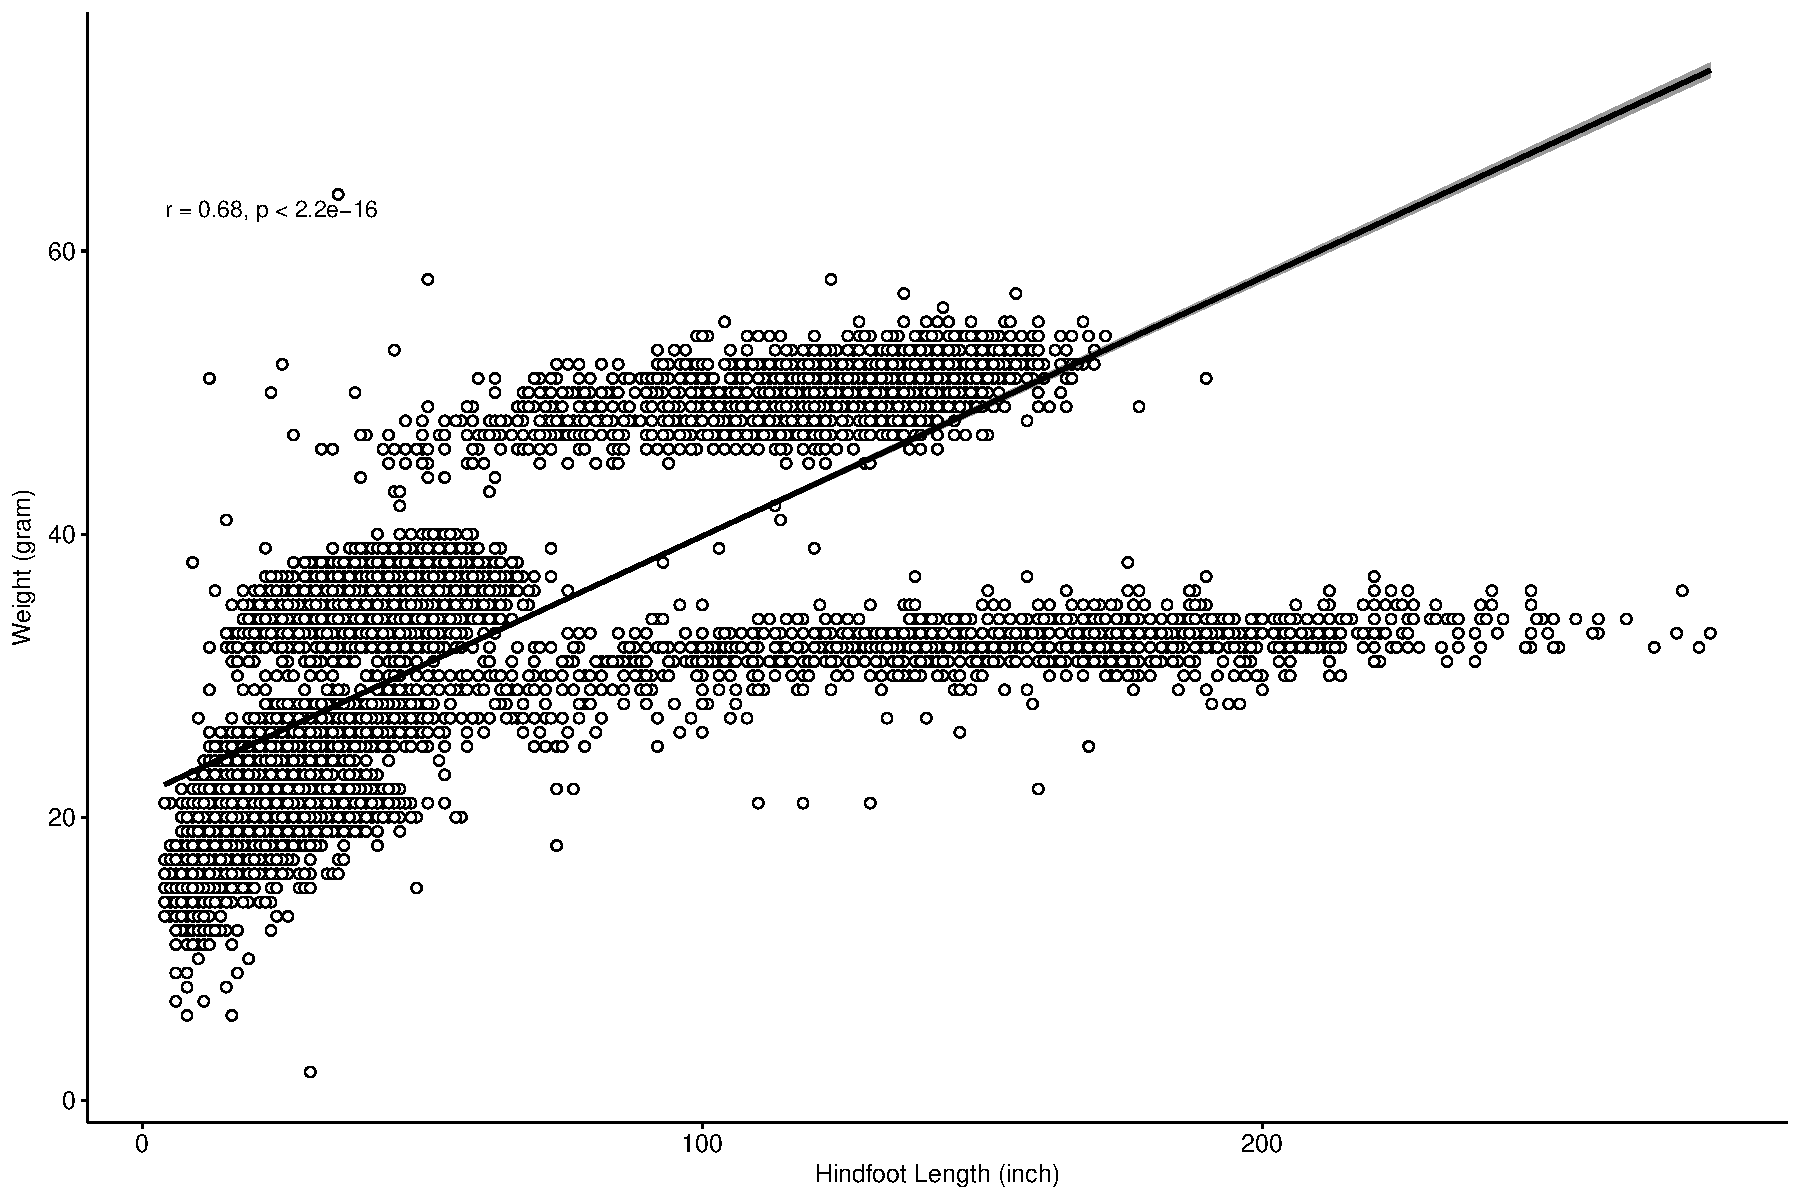
\includegraphics{figs/weight_and_hindfoot_length-1.pdf} Figure 3:
Scatter plot showing the correlation between weight and hindfoot length
of different species

The p-value of the test is less than the significance level alpha =
0.05. We can conclude that weight and hindfoot length are significantly
positively correlated with a correlation coefficient of 0.68 and p-value
of 2.2*10\^{}\{-16\}

\section{4. Hindfoot length of different
species}\label{hindfoot-length-of-different-species}

\begin{Shaded}
\begin{Highlighting}[]
\KeywordTok{ggplot}\NormalTok{(surveys_NAsrem, }\KeywordTok{aes}\NormalTok{(}\DataTypeTok{x =}\NormalTok{ species_id, }\DataTypeTok{y =}\NormalTok{ hindfoot_length)) }\OperatorTok{+}
\StringTok{  }\KeywordTok{geom_boxplot}\NormalTok{(}\DataTypeTok{alpha=}\DecValTok{1}\NormalTok{, }\DataTypeTok{color=} \StringTok{'black'}\NormalTok{)}\OperatorTok{+}\KeywordTok{xlab}\NormalTok{(}\StringTok{'Species ID'}\NormalTok{)}\OperatorTok{+}\KeywordTok{ylab}\NormalTok{(}\StringTok{'Hindfoot length (inch)'}\NormalTok{)}\OperatorTok{+}
\StringTok{  }\KeywordTok{stat_summary}\NormalTok{(}\DataTypeTok{fun.y=}\NormalTok{mean, }\DataTypeTok{color=}\StringTok{"blue"}\NormalTok{, }\DataTypeTok{geom=}\StringTok{"point"}\NormalTok{,  }\DataTypeTok{shape=}\DecValTok{15}\NormalTok{, }\DataTypeTok{size=}\DecValTok{1}\NormalTok{,}\DataTypeTok{show_guide =}\NormalTok{ T,}\DataTypeTok{show.legend =}\NormalTok{ T)}\OperatorTok{+}\StringTok{ }\KeywordTok{theme}\NormalTok{(}\DataTypeTok{axis.text.x =} \KeywordTok{element_text}\NormalTok{(}\DataTypeTok{angle =} \DecValTok{90}\NormalTok{))}
\end{Highlighting}
\end{Shaded}

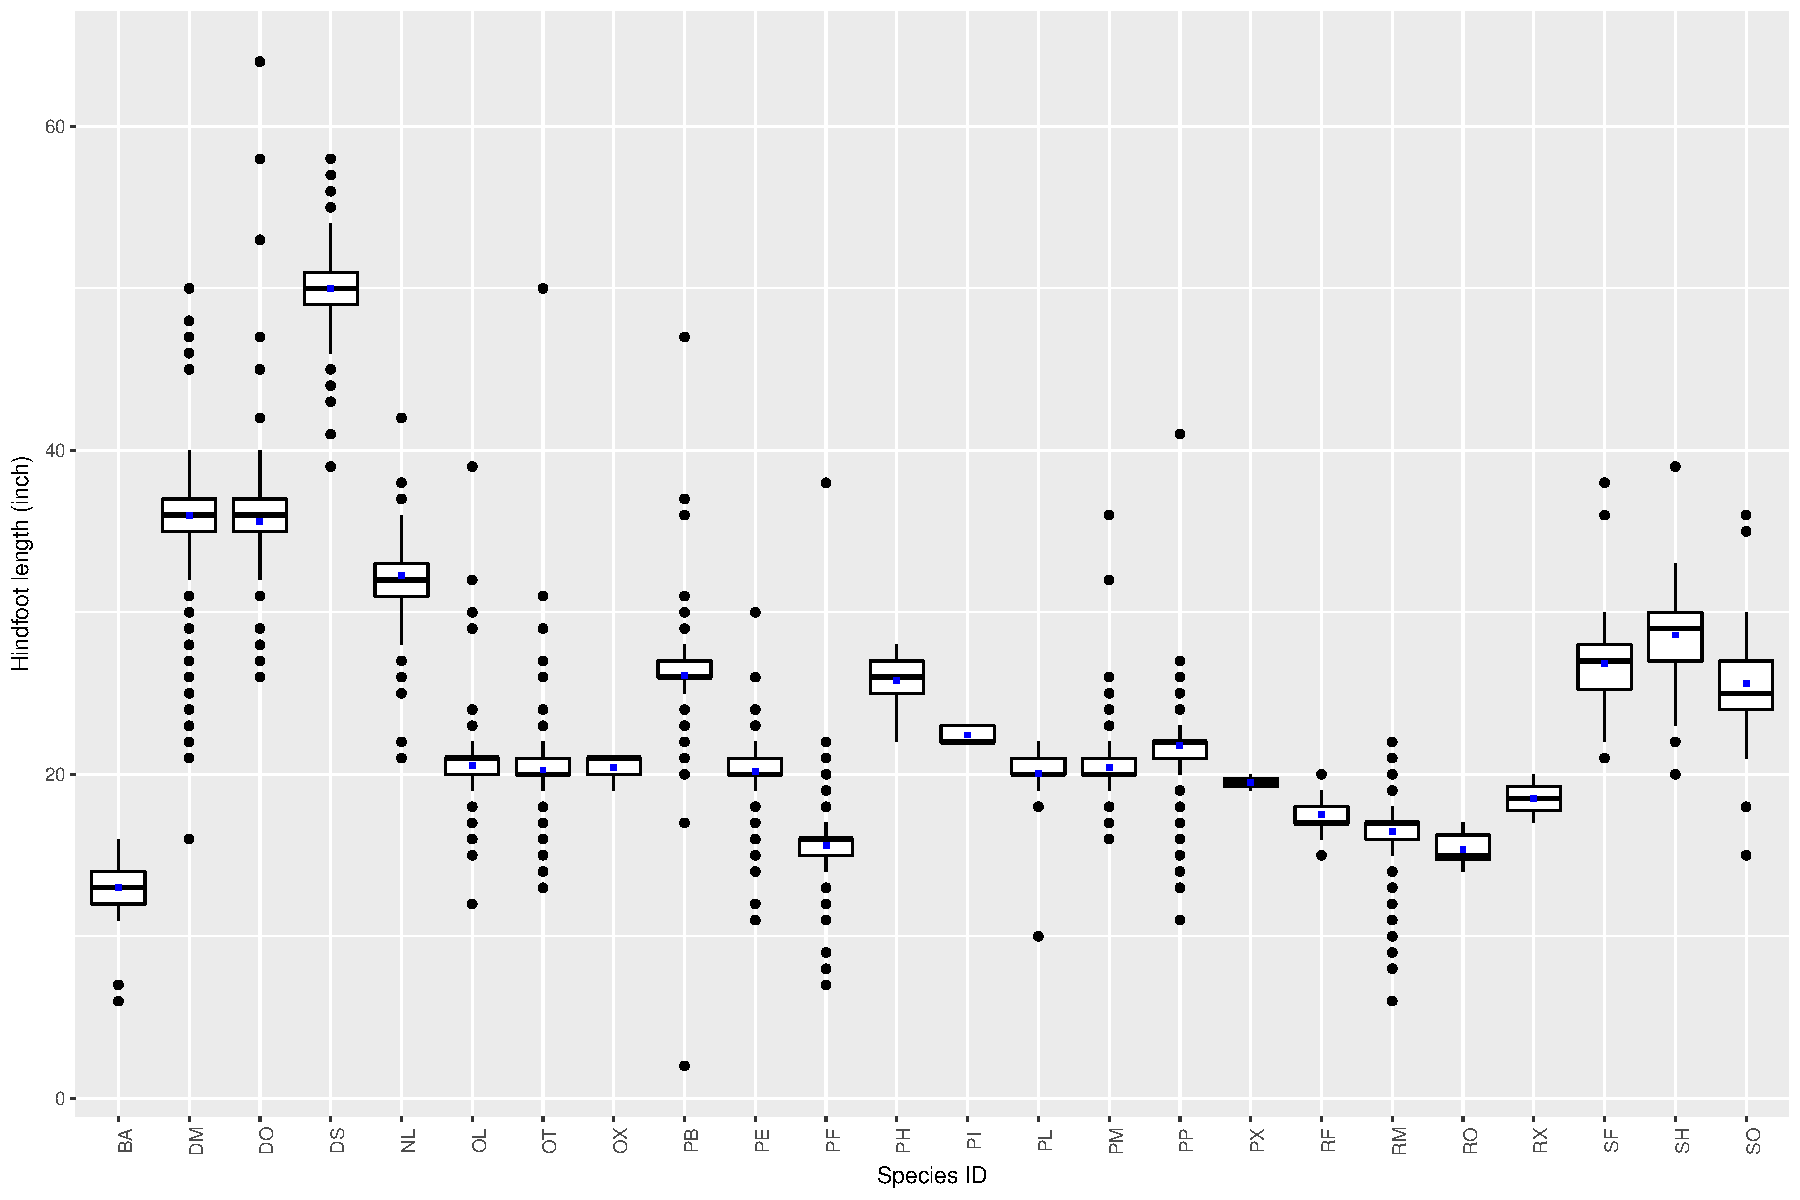
\includegraphics{figs/boxplot_hindfoot_lengths_different_species-1.pdf}
Figure 4: Box plot of hindfoot length of different species. The blue dot
indicates the average (mean) hindfoot length.

\section{5 Number of species found
yearly}\label{number-of-species-found-yearly}

\begin{Shaded}
\begin{Highlighting}[]
\NormalTok{yearly_counts <-}\StringTok{ }\NormalTok{surveys_NAsrem }\OperatorTok\StringTok{ }\KeywordTok{group_by}\NormalTok{(year, species_id) }\OperatorTok\StringTok{ }\KeywordTok{tally}\NormalTok{()}
\KeywordTok{ggplot}\NormalTok{(}\DataTypeTok{data =}\NormalTok{ yearly_counts, }\KeywordTok{aes}\NormalTok{(}\DataTypeTok{x=}\NormalTok{year, }\DataTypeTok{y=}\NormalTok{n, }\DataTypeTok{group =}\NormalTok{ species_id, }\DataTypeTok{color =}\NormalTok{ species_id)) }\OperatorTok{+}\StringTok{ }
\StringTok{  }\KeywordTok{geom_line}\NormalTok{() }\OperatorTok{+}\StringTok{ }\KeywordTok{facet_wrap}\NormalTok{(}\OperatorTok{~}\StringTok{ }\NormalTok{species_id) }\OperatorTok{+}\StringTok{ }\KeywordTok{theme_bw}\NormalTok{() }\OperatorTok{+}\KeywordTok{ylab}\NormalTok{(}\StringTok{'Number of Individuals'}\NormalTok{) }\OperatorTok{+}\StringTok{ }\KeywordTok{xlab}\NormalTok{(}\StringTok{'Year'}\NormalTok{)}
\end{Highlighting}
\end{Shaded}

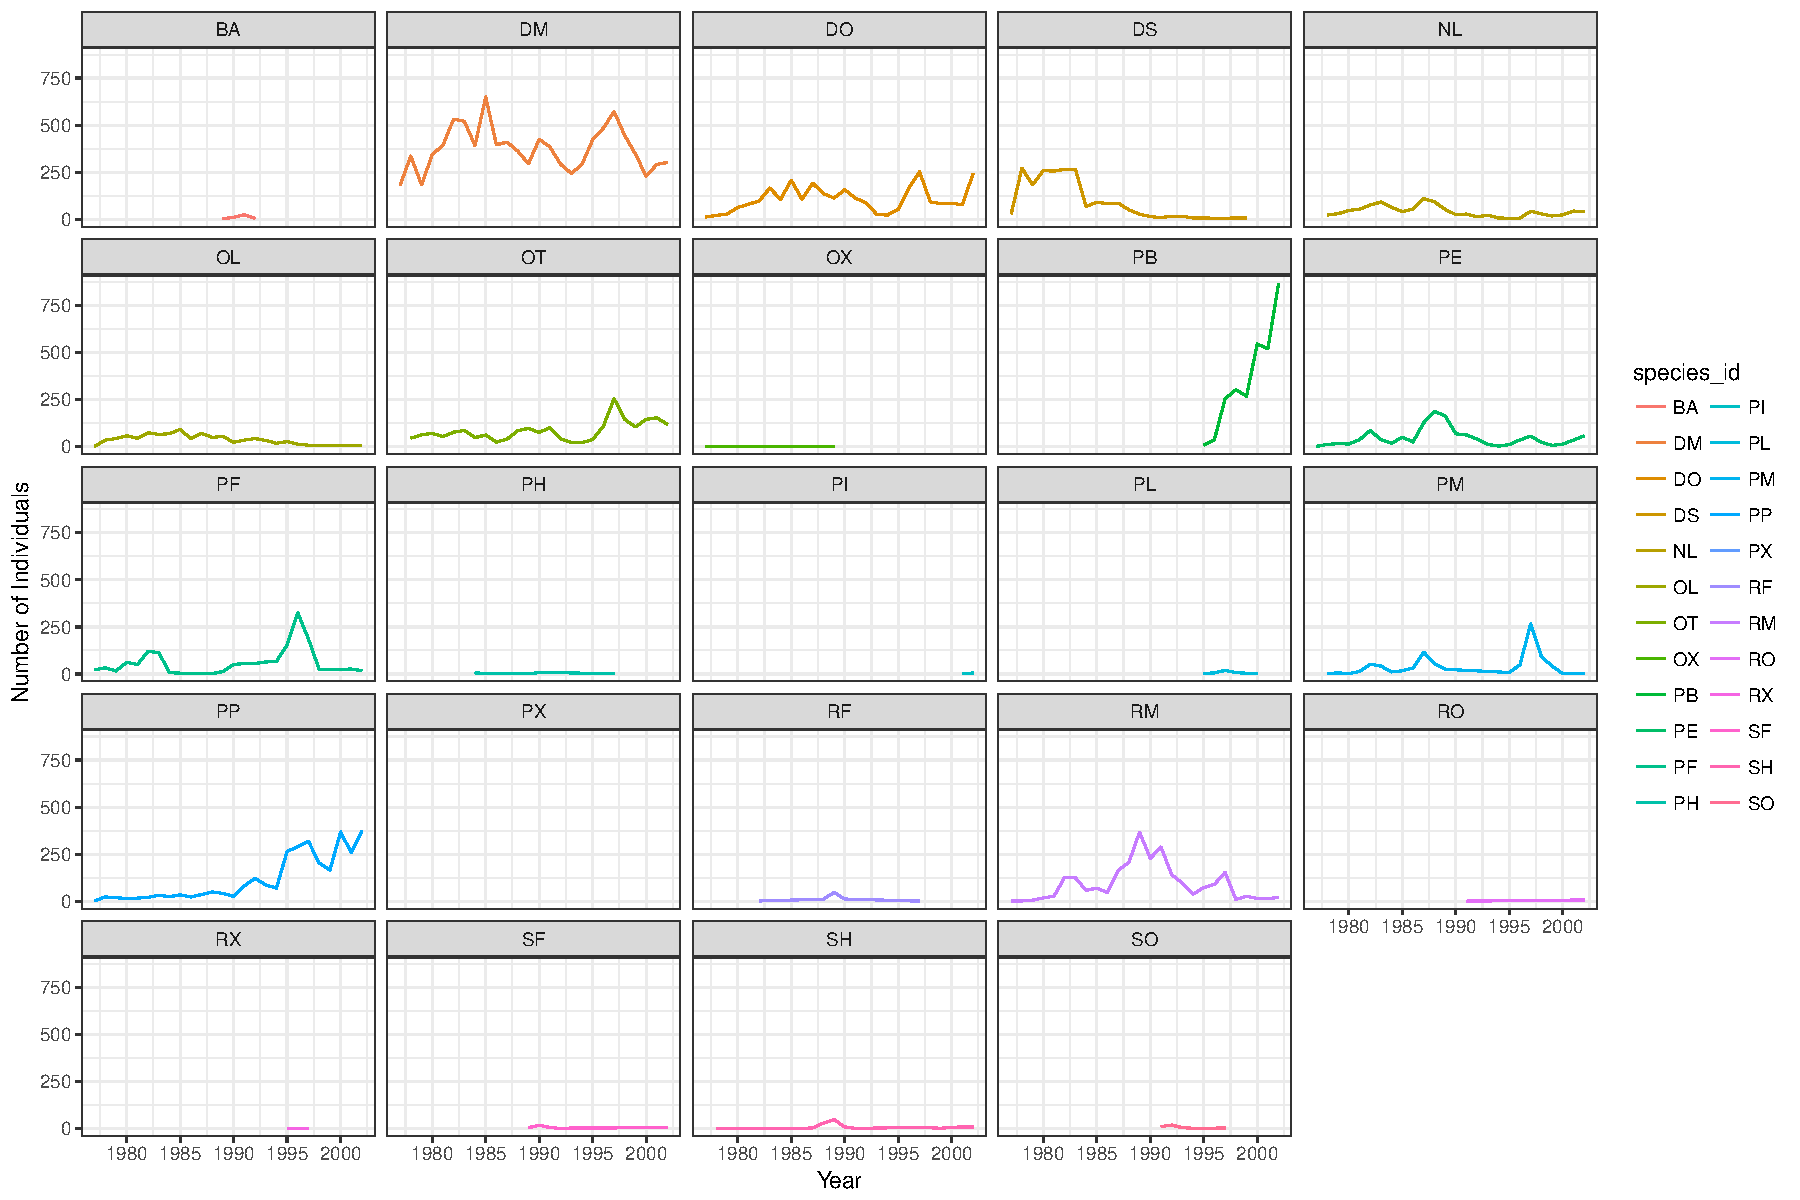
\includegraphics{figs/species_count-1.pdf} Figure 5: Time series
faceting plot showing the count of each species yearly.

\section{6 Number of species found in each plot
type}\label{number-of-species-found-in-each-plot-type}

\begin{Shaded}
\begin{Highlighting}[]
\NormalTok{Plot_counts <-}\StringTok{ }\NormalTok{surveys_NAsrem }\OperatorTok\StringTok{ }\KeywordTok{group_by}\NormalTok{(year, plot_type) }\OperatorTok\StringTok{ }\KeywordTok{tally}\NormalTok{()}
\KeywordTok{ggplot}\NormalTok{(Plot_counts, }\KeywordTok{aes}\NormalTok{(}\DataTypeTok{x=}\NormalTok{year, }\DataTypeTok{y=}\NormalTok{n, }\DataTypeTok{color=}\NormalTok{plot_type)) }\OperatorTok{+}\StringTok{ }\KeywordTok{geom_point}\NormalTok{()}\OperatorTok{+}\KeywordTok{facet_wrap}\NormalTok{(}\OperatorTok{~}\NormalTok{plot_type)}
\end{Highlighting}
\end{Shaded}

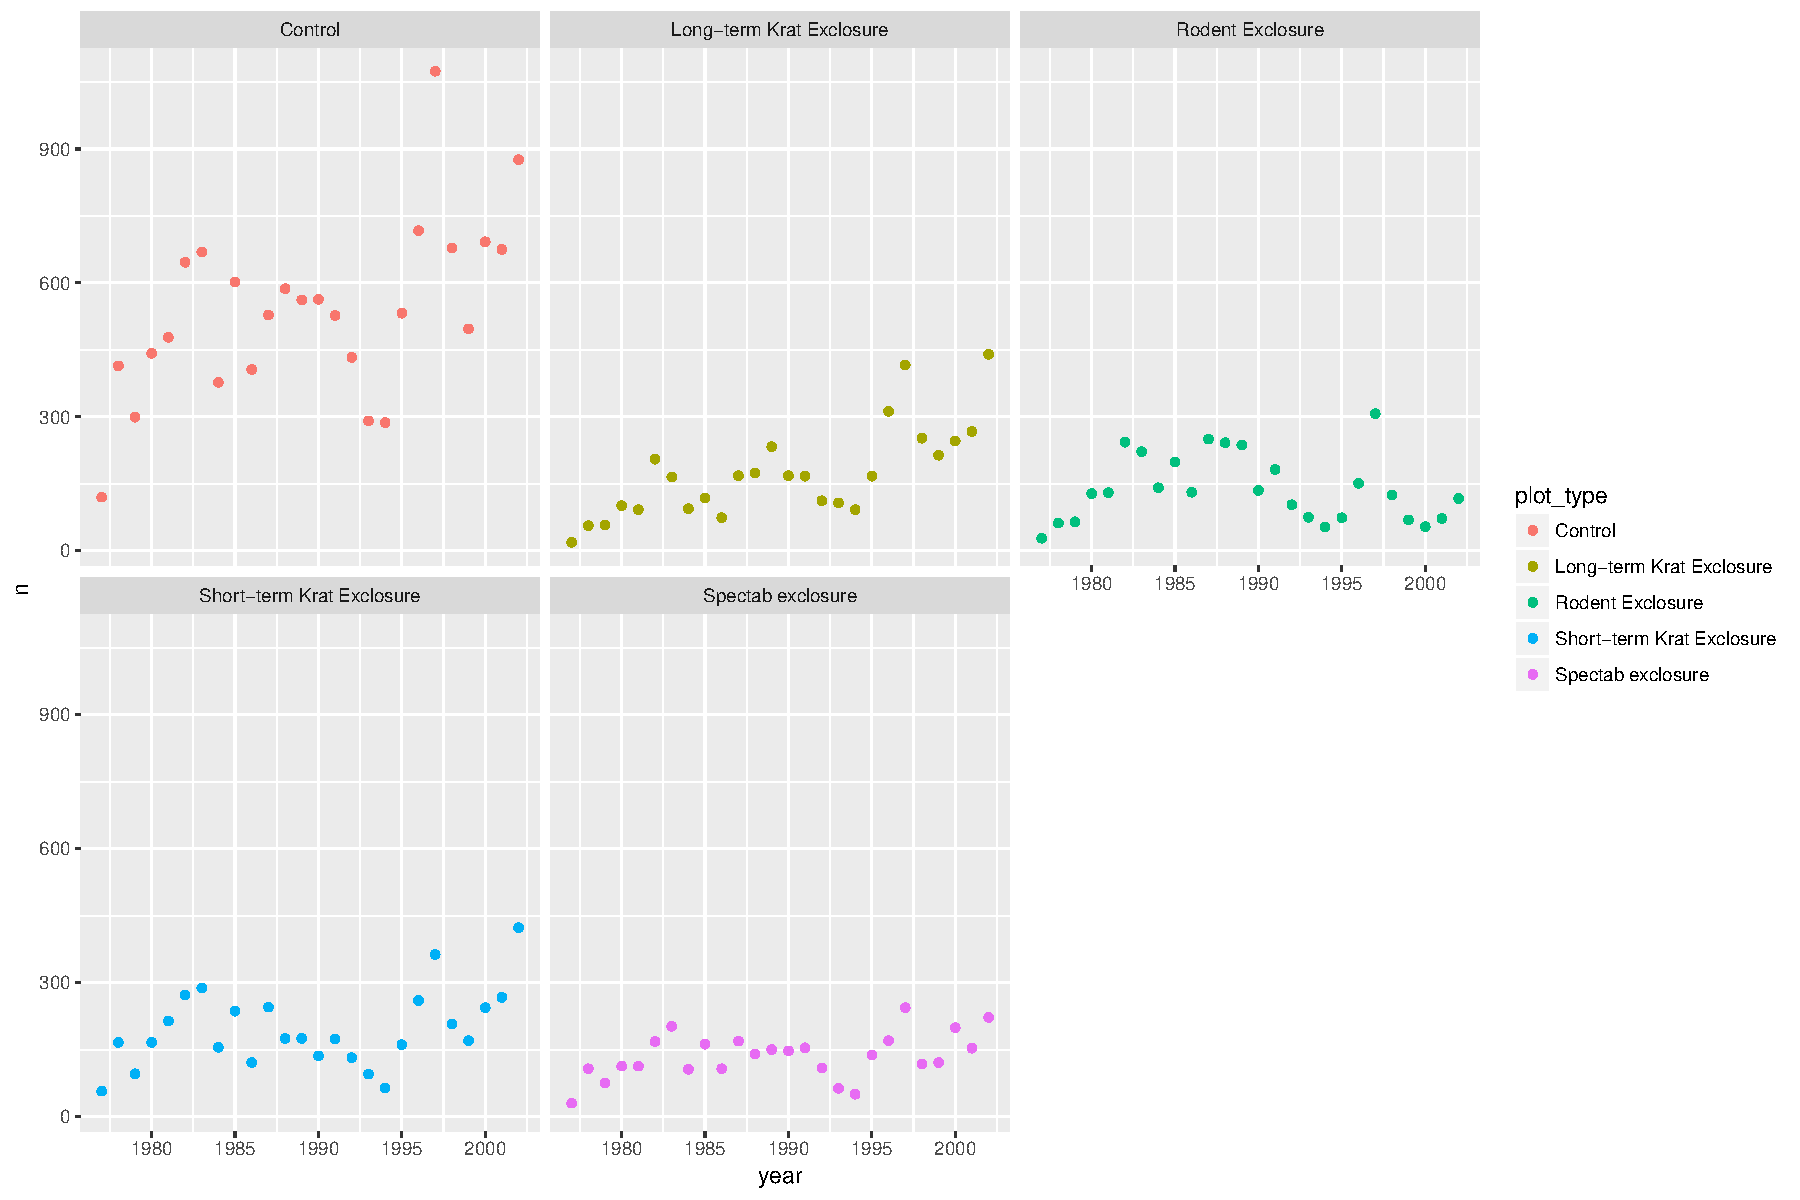
\includegraphics{figs/species_count_by_plot-1.pdf} Figure 6: time series
faceting plot showing the count of species observed in each plot type
yearly.

\section{7 Males and females average weight yearly
PROBLEMS}\label{males-and-females-average-weight-yearly-problems}

\begin{Shaded}
\begin{Highlighting}[]
\CommentTok{# Species mean weight *********}
\NormalTok{spe_meanweight <-}\StringTok{ }\NormalTok{surveys_NAsrem }\OperatorTok\StringTok{ }\KeywordTok{group_by}\NormalTok{(year,species_id, sex) }\OperatorTok
\StringTok{  }\KeywordTok{mutate}\NormalTok{(}\DataTypeTok{mean_weight =} \KeywordTok{mean}\NormalTok{(weight))}
\CommentTok{# plot}
\KeywordTok{ggplot}\NormalTok{(spe_meanweight, }\KeywordTok{aes}\NormalTok{(}\DataTypeTok{x=}\NormalTok{year, }\DataTypeTok{y=}\NormalTok{mean_weight, }\DataTypeTok{color=}\NormalTok{sex)) }\OperatorTok{+}
\StringTok{  }\KeywordTok{geom_line}\NormalTok{()}\OperatorTok{+}\KeywordTok{facet_wrap}\NormalTok{(}\OperatorTok{~}\NormalTok{species_id) }\OperatorTok{+}\StringTok{ }\KeywordTok{theme_bw}\NormalTok{() }\OperatorTok{+}
\StringTok{  }\KeywordTok{theme}\NormalTok{(}\DataTypeTok{panel.grid =} \KeywordTok{element_blank}\NormalTok{()) }\OperatorTok{+}
\StringTok{  }\KeywordTok{theme}\NormalTok{(}\DataTypeTok{axis.text.x =} \KeywordTok{element_text}\NormalTok{(}\DataTypeTok{colour =} \StringTok{"grey20"}\NormalTok{, }\DataTypeTok{size =} \DecValTok{10}\NormalTok{, }\DataTypeTok{angle =} \DecValTok{90}\NormalTok{, }\DataTypeTok{hjust =} \FloatTok{0.5}\NormalTok{, }\DataTypeTok{vjust =} \FloatTok{0.5}\NormalTok{))}
\end{Highlighting}
\end{Shaded}

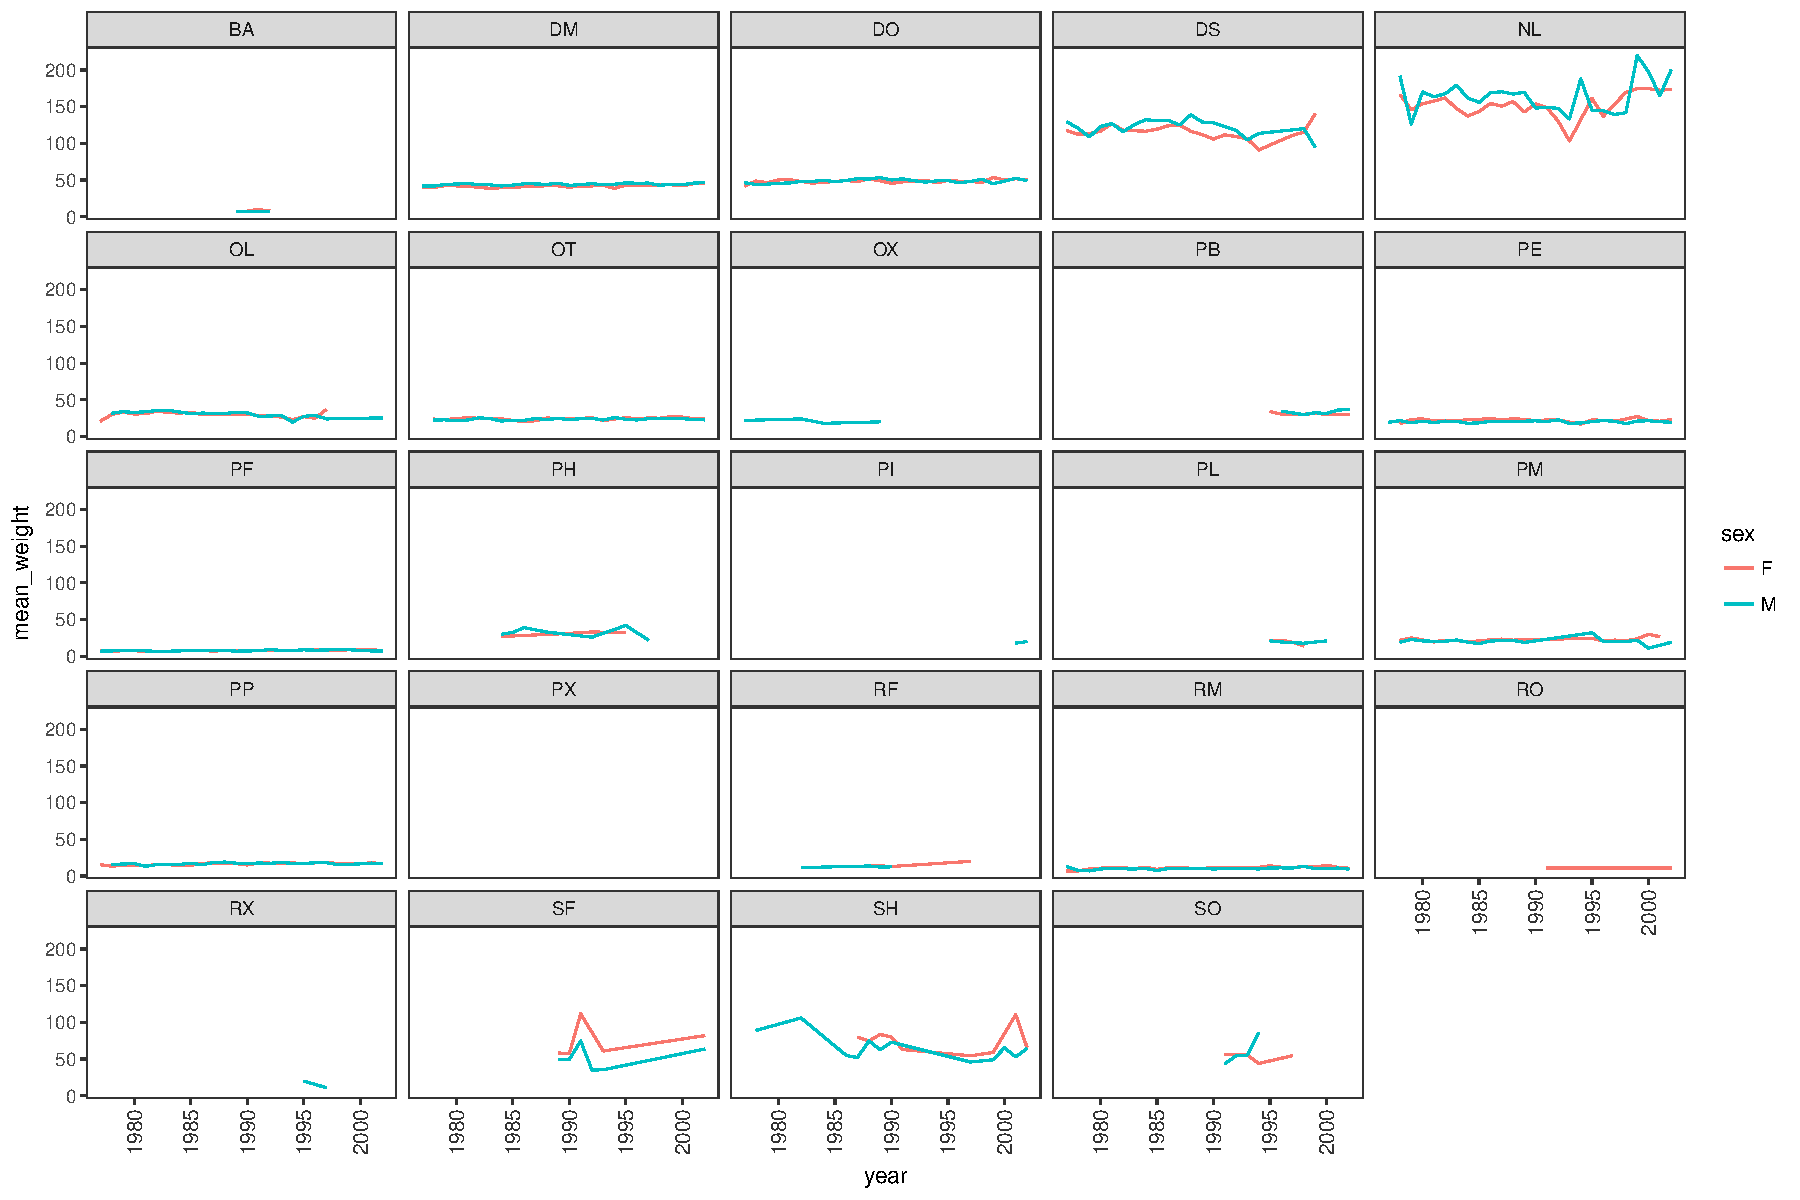
\includegraphics{figs/Sex_average_weight-1.pdf} Figure 7: time series
faceting plot showing yearly average weight of each male and female
species.

\section{8 Count of species observed}\label{count-of-species-observed}

\begin{Shaded}
\begin{Highlighting}[]
\KeywordTok{ggplot}\NormalTok{(surveys_NAsrem) }\OperatorTok{+}\StringTok{ }\KeywordTok{stat_count}\NormalTok{(}\KeywordTok{aes}\NormalTok{(}\DataTypeTok{x =}\NormalTok{ species_id, }\DataTypeTok{fill =}\NormalTok{ species_id))}
\end{Highlighting}
\end{Shaded}

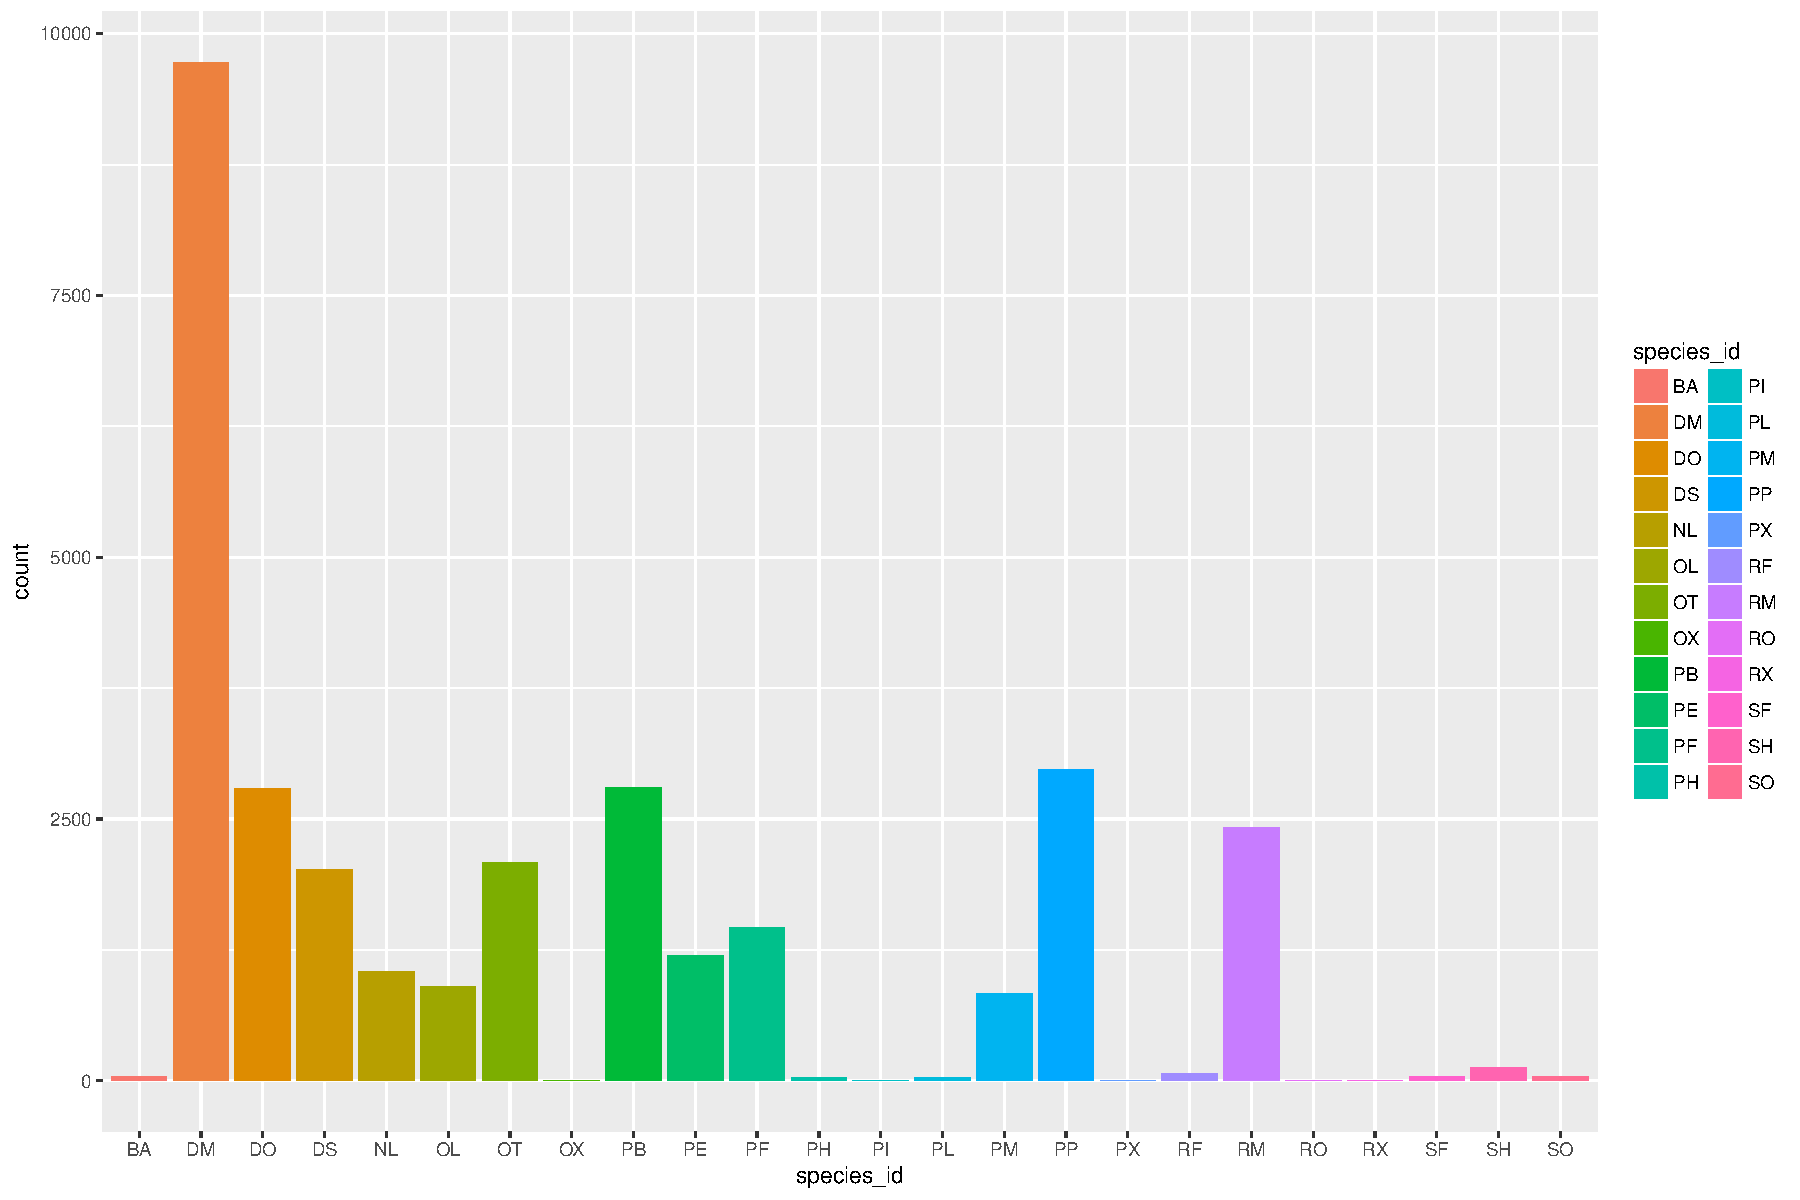
\includegraphics{figs/bar_chart_individuals_each_species-1.pdf} Figure
8: Bar graph showing number of individuals of each species obeserved.

\section{9 Number of individuals of each sex by species
surveyed}\label{number-of-individuals-of-each-sex-by-species-surveyed}

\begin{Shaded}
\begin{Highlighting}[]
\KeywordTok{ggplot}\NormalTok{(surveys_NAsrem) }\OperatorTok{+}\StringTok{ }\KeywordTok{stat_count}\NormalTok{(}\KeywordTok{aes}\NormalTok{(}\DataTypeTok{x =}\NormalTok{ species_id, }\DataTypeTok{fill =}\NormalTok{ sex), }\DataTypeTok{position =} \StringTok{"dodge"}\NormalTok{)}
\end{Highlighting}
\end{Shaded}

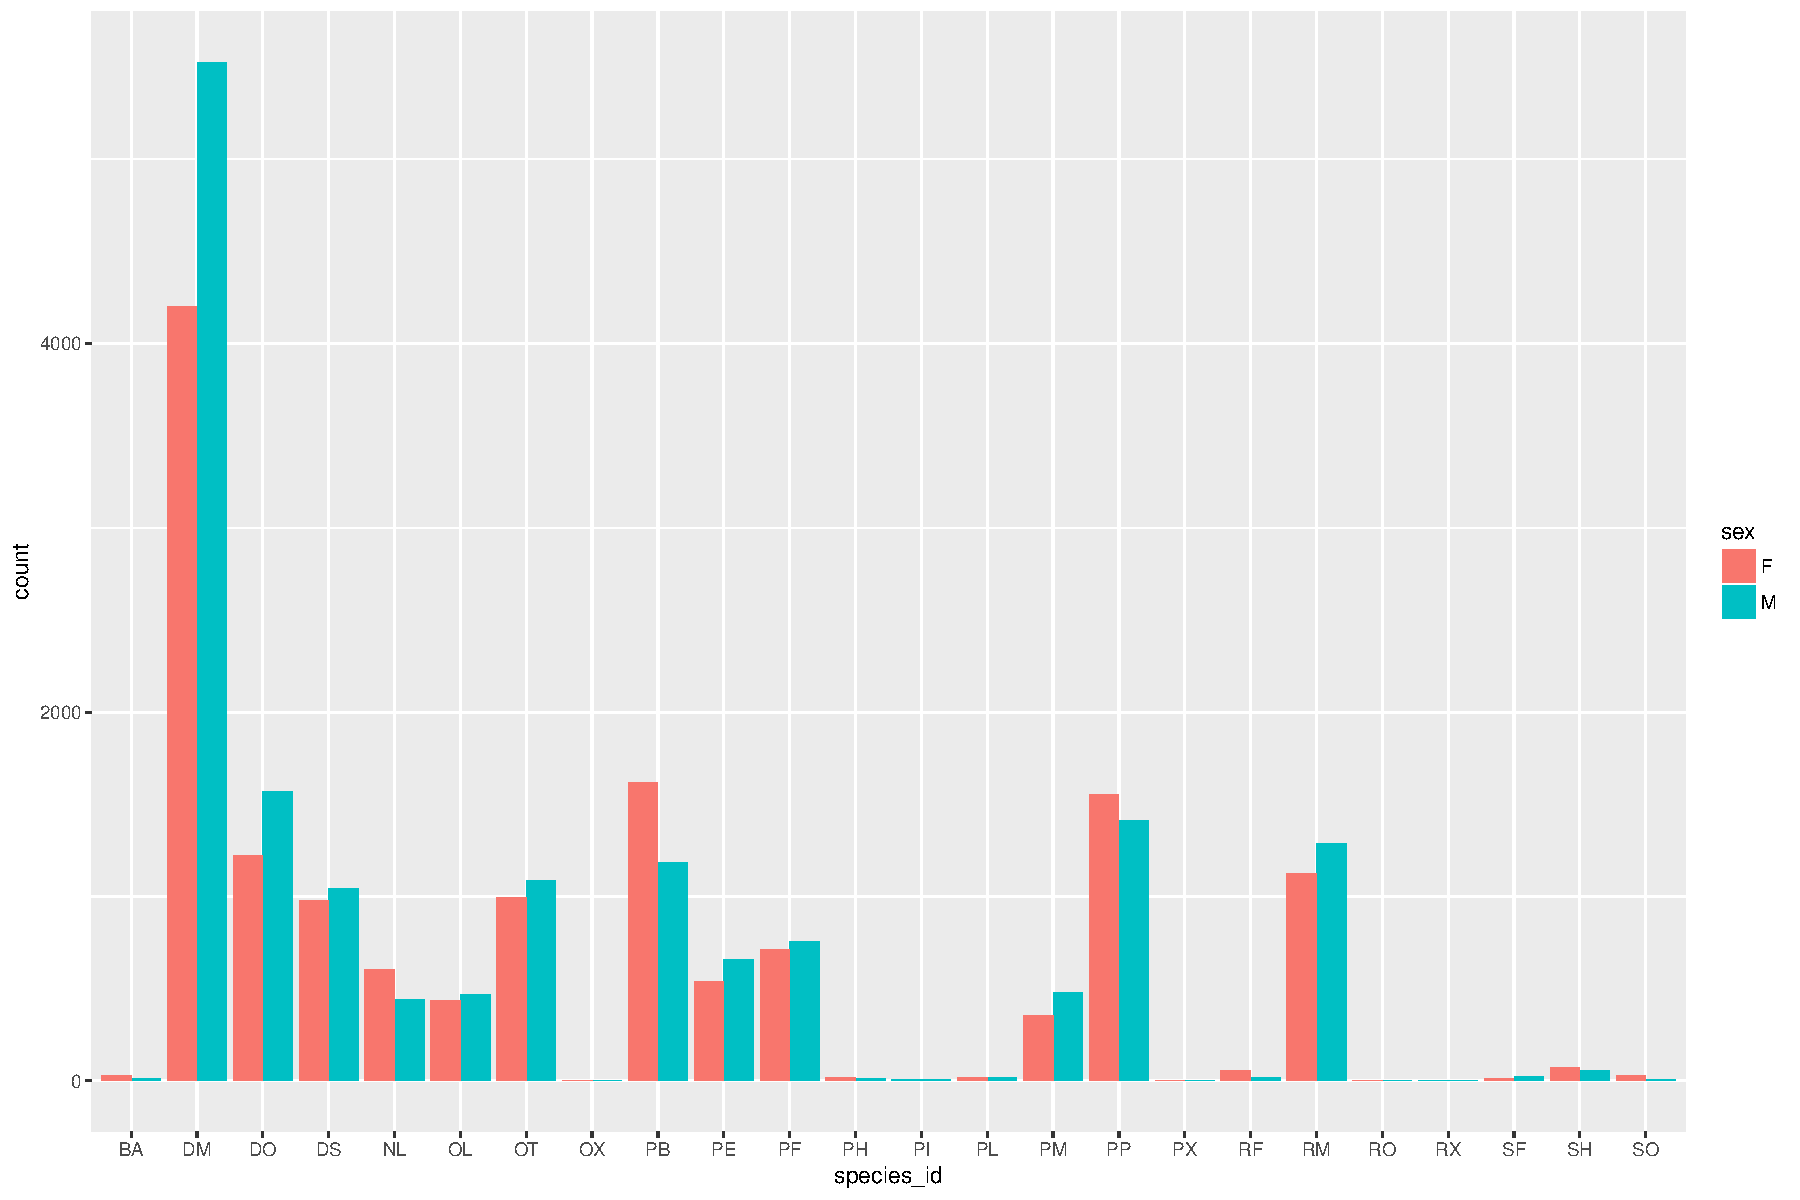
\includegraphics{figs/number_individuals_species_sex-1.pdf} Figure 9:
Number of individuals of each sex by species surveyed.

\section{10 relationship between species weight and
sex}\label{relationship-between-species-weight-and-sex}

\begin{Shaded}
\begin{Highlighting}[]
\CommentTok{#this one looks a little weird, gotta play around with it }
\KeywordTok{ggplot}\NormalTok{(surveys_NAsrem) }\OperatorTok{+}\StringTok{ }\KeywordTok{geom_boxplot}\NormalTok{(}\KeywordTok{aes}\NormalTok{(}\DataTypeTok{x =}\NormalTok{ species_id, }\DataTypeTok{y =}\NormalTok{ weight, }\DataTypeTok{fill =}\NormalTok{ sex)) }\OperatorTok{+}
\StringTok{  }\KeywordTok{coord_flip}\NormalTok{()}
\end{Highlighting}
\end{Shaded}

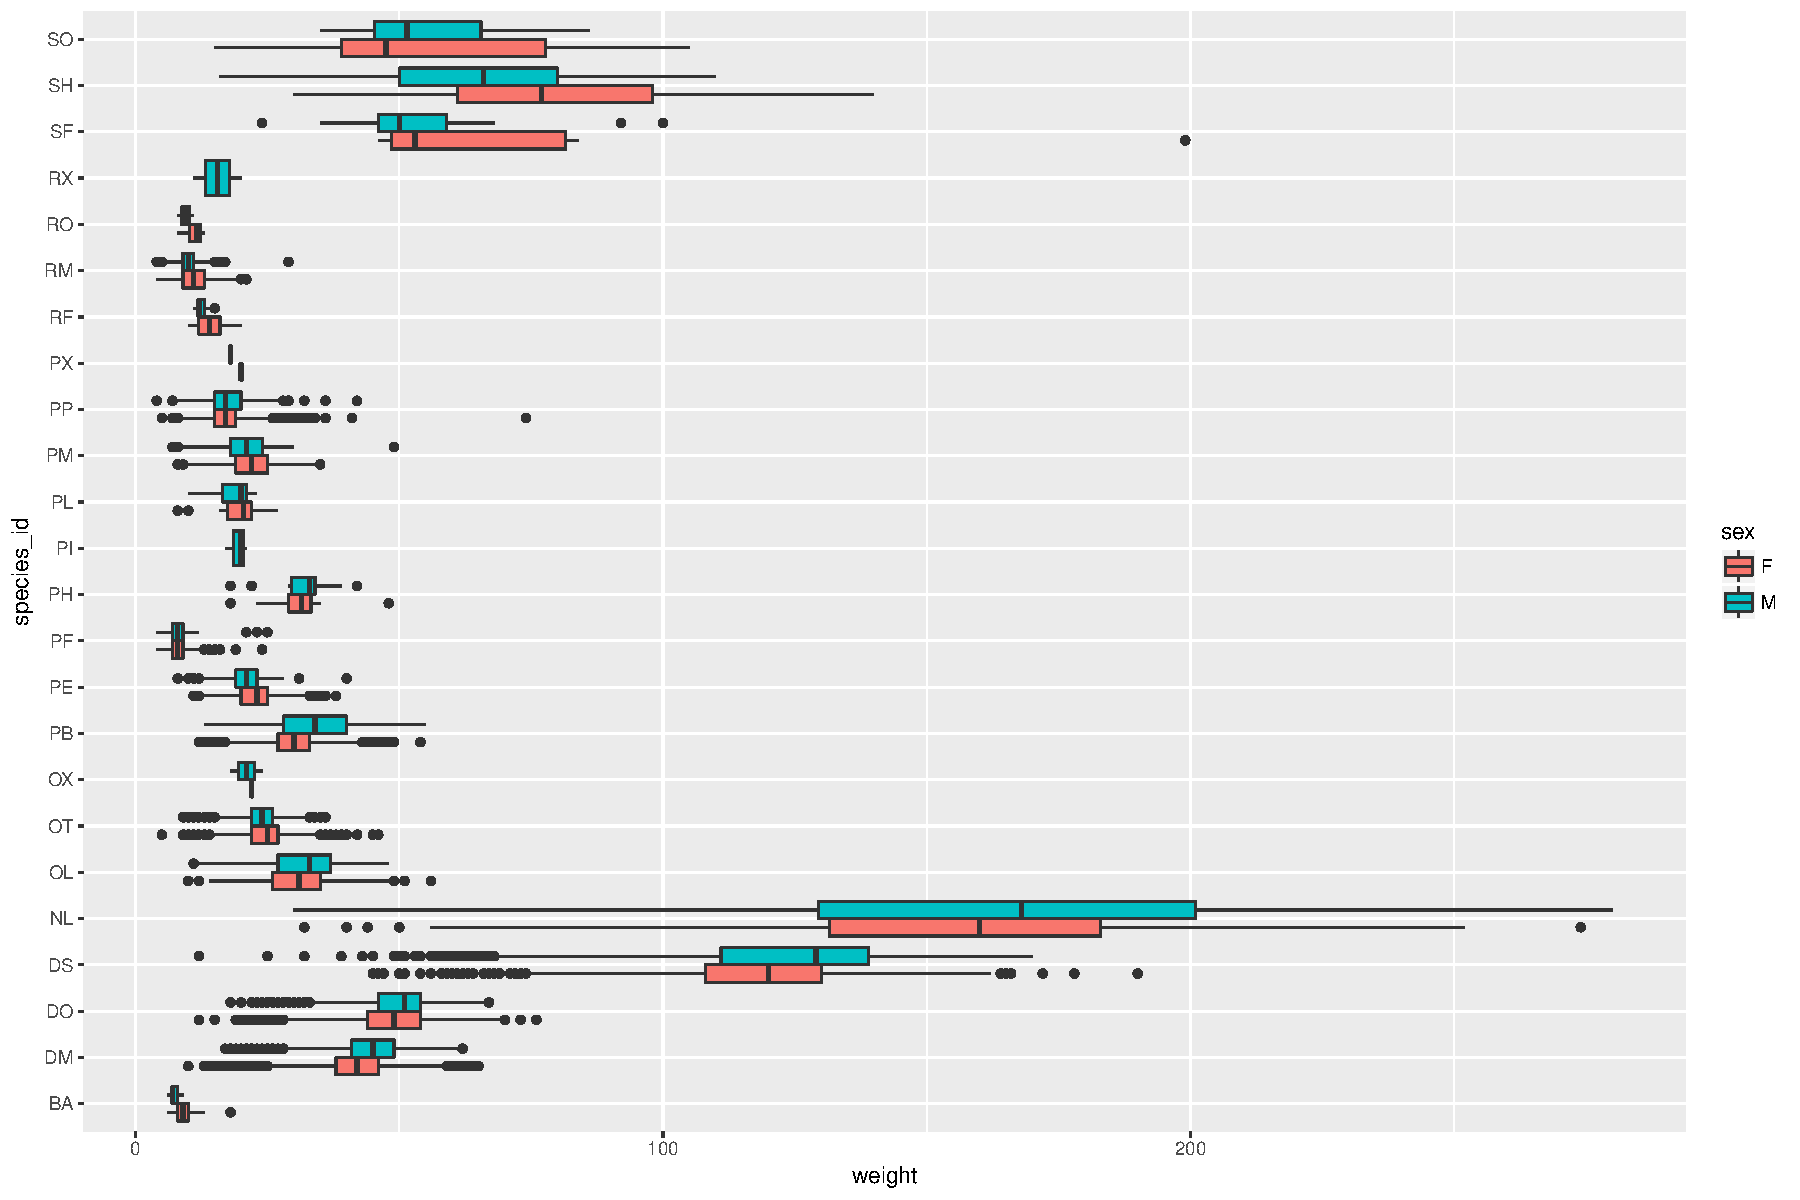
\includegraphics{figs/weight_sex-1.pdf} Figure 10: Box plot (axis
fliped) showing the relationship between species sex and weight

\section{11 Number of individuals seen over time, separated by
sex}\label{number-of-individuals-seen-over-time-separated-by-sex}

\begin{Shaded}
\begin{Highlighting}[]
\NormalTok{yearly_sex_counts <-}\StringTok{ }\NormalTok{surveys_NAsrem }\OperatorTok\StringTok{ }\KeywordTok{group_by}\NormalTok{(year, species_id, sex) }\OperatorTok
\StringTok{  }\NormalTok{tally}
\KeywordTok{ggplot}\NormalTok{(}\DataTypeTok{data =}\NormalTok{ yearly_sex_counts, }\KeywordTok{aes}\NormalTok{(}\DataTypeTok{x =}\NormalTok{ year, }\DataTypeTok{y =}\NormalTok{ n, }\DataTypeTok{color =}\NormalTok{ sex, }\DataTypeTok{group =}\NormalTok{ sex)) }\OperatorTok{+}
\StringTok{  }\KeywordTok{geom_line}\NormalTok{() }\OperatorTok{+}
\StringTok{  }\KeywordTok{facet_wrap}\NormalTok{(}\OperatorTok{~}\StringTok{ }\NormalTok{species_id) }\OperatorTok{+}
\StringTok{  }\KeywordTok{theme_bw}\NormalTok{() }\OperatorTok{+}\KeywordTok{ylab}\NormalTok{(}\StringTok{'Number of Individuals'}\NormalTok{) }\OperatorTok{+}\StringTok{ }\KeywordTok{xlab}\NormalTok{(}\StringTok{'Year'}\NormalTok{)}\OperatorTok{+}\StringTok{ }\KeywordTok{theme}\NormalTok{(}\DataTypeTok{axis.text.x =} \KeywordTok{element_text}\NormalTok{(}\DataTypeTok{angle =} \DecValTok{90}\NormalTok{))}
\end{Highlighting}
\end{Shaded}

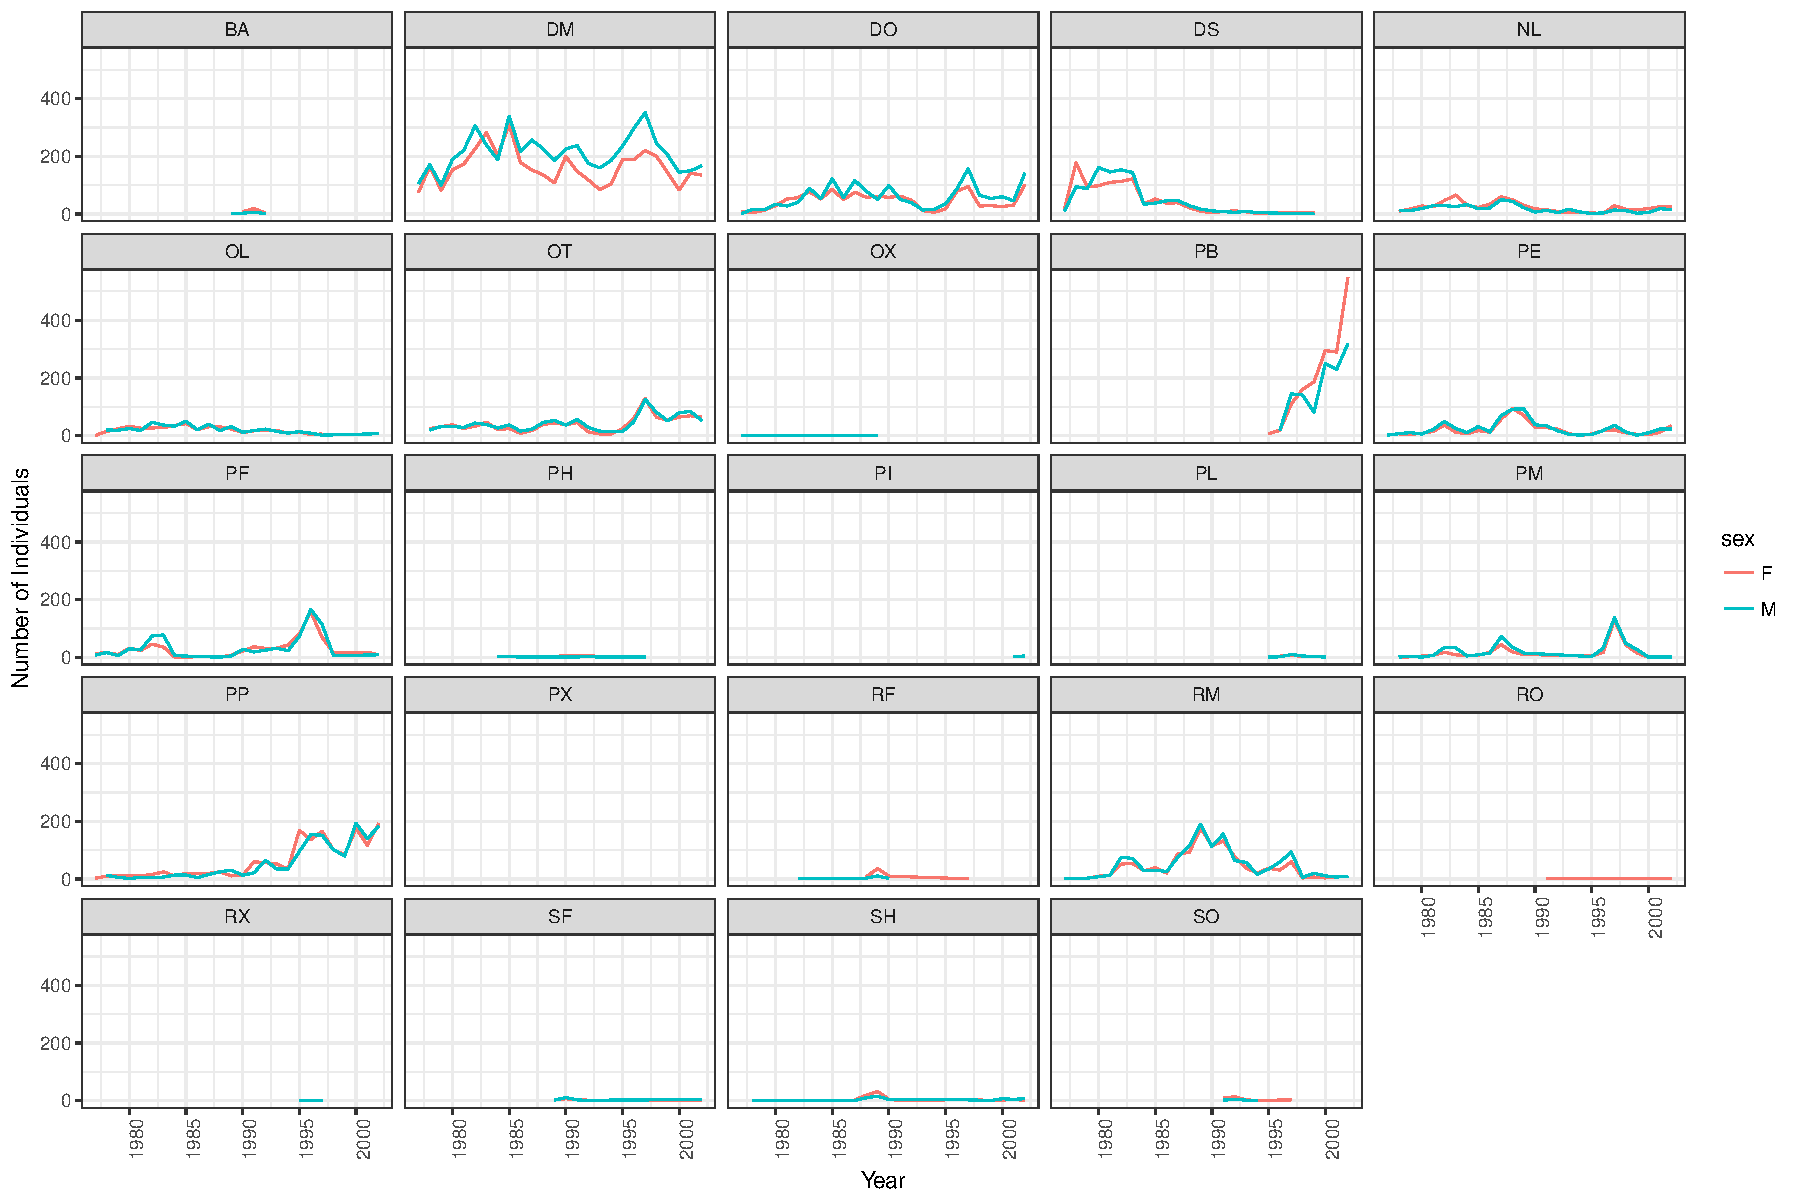
\includegraphics{figs/individuals_sex_over_time-1.pdf} Figure 11: Number
of individuals of each sex seen over time, separated by species

\section{12 Relationship between hindfoot length and weight of species
OT}\label{relationship-between-hindfoot-length-and-weight-of-species-ot}

\begin{Shaded}
\begin{Highlighting}[]
\NormalTok{species_OT <-}\StringTok{ }\NormalTok{surveys_NAsrem }\OperatorTok\StringTok{ }\KeywordTok{filter}\NormalTok{(species_id }\OperatorTok{==}\StringTok{ 'OT'}\NormalTok{)}
\KeywordTok{ggscatter}\NormalTok{(species_OT, }\DataTypeTok{x =} \StringTok{"weight"}\NormalTok{, }\DataTypeTok{y =} \StringTok{"hindfoot_length"}\NormalTok{, }\DataTypeTok{color =} \StringTok{"black"}\NormalTok{, }\DataTypeTok{shape =} \DecValTok{21}\NormalTok{, }\DataTypeTok{size =} \DecValTok{2}\NormalTok{, }\DataTypeTok{add =} \StringTok{"reg.line"}\NormalTok{, }\DataTypeTok{conf.int =} \OtherTok{TRUE}\NormalTok{, }
          \DataTypeTok{cor.coef =} \OtherTok{TRUE}\NormalTok{, }\DataTypeTok{cor.method =} \StringTok{"pearson"}\NormalTok{,  }\DataTypeTok{xlab =} \StringTok{"Hindfoot Length (inch)"}\NormalTok{, }\DataTypeTok{ylab =} \StringTok{"Weight (gram)"}\NormalTok{)}
\end{Highlighting}
\end{Shaded}

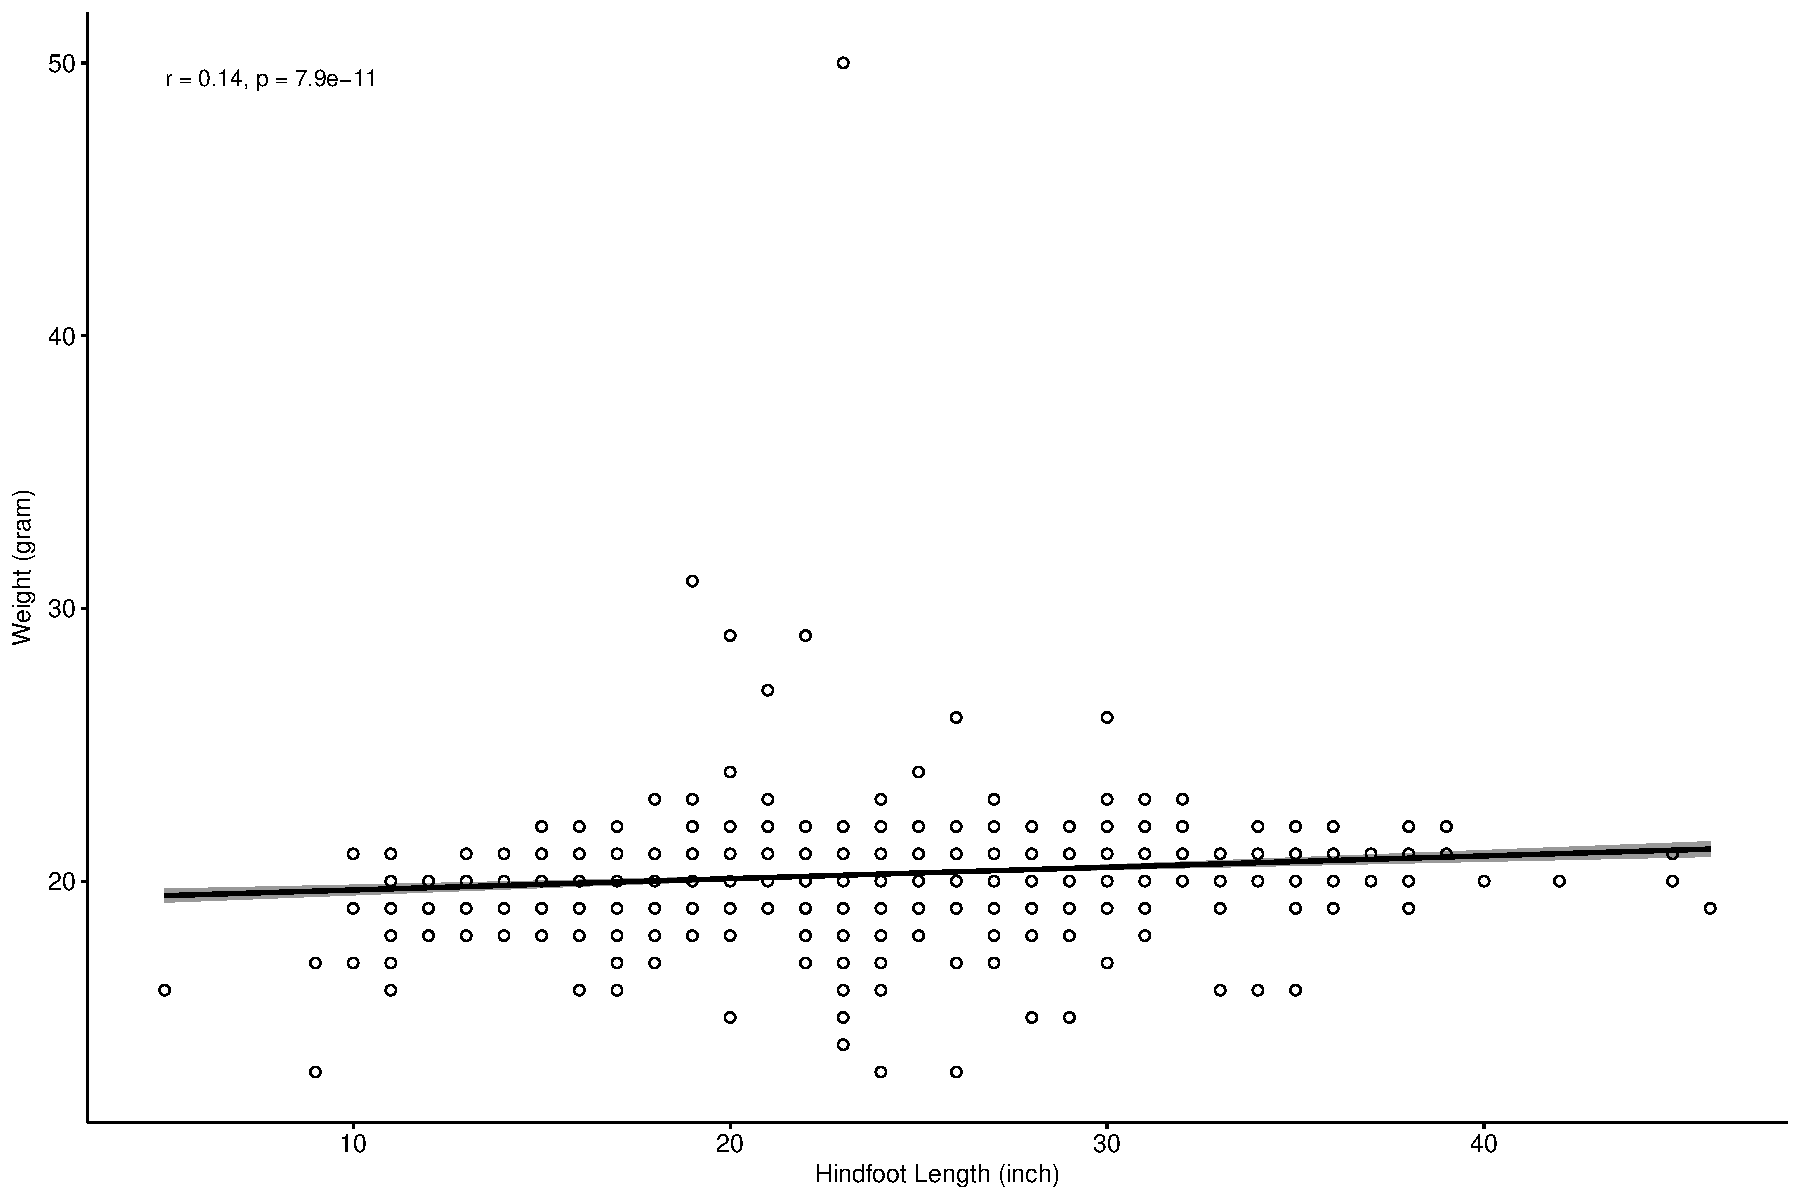
\includegraphics{figs/OT_weight_hindfoot_length-1.pdf} Figure 12:
Relationship between hindfoot length and weight of individuals for
species OT.


\end{document}
